\documentclass[12pt]{article}
\usepackage{hyperref}

\usepackage{amsmath}
\usepackage{graphicx,psfrag,epsf}
\usepackage{enumerate}
\usepackage{natbib}
\usepackage{url} % not crucial - just used below for the URL

%\pdfminorversion=4
% NOTE: To produce blinded version, replace "0" with "1" below.
\newcommand{\blind}{0}

% DON'T change margins - should be 1 inch all around.
\addtolength{\oddsidemargin}{-.5in}%
\addtolength{\evensidemargin}{-.5in}%
\addtolength{\textwidth}{1in}%
\addtolength{\textheight}{1.3in}%
\addtolength{\topmargin}{-.8in}%

\begin{document}

\def\spacingset#1{\renewcommand{\baselinestretch}%
{#1}\small\normalsize} \spacingset{1}


%%%%%%%%%%%%%%%%%%%%%%%%%%%%%%%%%%%%%%%%%%%%%%%%%%%%%%%%%%%%%%%%%%%%%%%%%%%%%%

\if0\blind
{
  \title{\bf Interactive Visualization of Hierarchically Structured Data}
  \author{Kris Sankaran\thanks{
      This research was supported in part by an NIH training grant (5T32GM096982-03) and a Weiland Fellowship.}\hspace{.2cm}\\
    Department of Statistics, Stanford University\\
    and \\
    Susan Holmes\thanks{
       This research was supported in part by NIH grant R01 AI112401.
      }\hspace{0.2cm}\\
    Department of Statistics, Stanford University}
  \maketitle
} \fi

\if1\blind
{
  \bigskip
  \bigskip
  \bigskip
  \begin{center}
    {\LARGE\bf Title}
\end{center}
  \medskip
} \fi

\bigskip
\begin{abstract}
We introduce methods for visualization of data structured along trees,
especially hierarchically structured collections of time series.  To
this end, we identify questions that often emerge when working with
hierarchical data and provide an R package to simplify their
investigation. Our key contribution is the adaptation of the
visualization principles of focus-plus-context and linking to the
study of tree-structured data.

Our motivating application is to the analysis of bacterial time
series, where an evolutionary tree relating bacteria is available a
priori. However, we have identified common problem types where, if a
tree is not directly available, it can be constructed from data and
then studied using our techniques. We perform detailed case studies to
describe the alternative use cases, interpretations, and utility of
the proposed visualization methods.

\end{abstract}

\noindent%
{\it Keywords:}  D3, focus-plus-context, linking, time-series, tree-structured, R
\vfill

\newpage
\spacingset{1.45} % DON'T change the spacing!

\subsection*{Introduction}\label{introduction}

We introduce methods for visualization of data structured along trees,
especially hierarchically structured collections of time series. We hope
both to characterize generically useful techniques for interactively
visualizing hierarchical data and to offer practical tools for
implementing such displays. To this end, we identify questions that
often emerge when working with hierarchical data and provide an R
package to simplify their investigation \citep{ihaka1996r}.

Our key contribution is the adaptation of the visualization principles
of focus-plus-context and linking to the study of tree-structured data
\citep{buja1996interactive, becker1987brushing}. Our motivating
application is to the analysis of bacterial time series, where an
evolutionary tree relating bacteria is available a priori. However, we
have identified common problem types where, if a tree is not directly
available, it can be constructed from data and then studied using our
techniques.

We have implemented our visualizations in D3, but encapsulated in an R
package, called treelapse, to facilitate rapid turnover from data
preparation and modeling to interactive exploration, and vice versa. Our
code is open-source, and available at
\url{https://github.com/krisrs1128/treelapse}\footnote{Link removed in blinded manuscript,
but available to editor.}. We hope this package encourages data analysts
to work at the border between data modeling and visualization, and more
generally empowers a wider audience to apply less widely known, but
powerful, visualization ideas.

The paper is organized as follows. First, we describe our motivating
application to the microbiome and the associated generic analysis tasks.
Next, we review the underlying visualization principles behind our
contributions. Then we then connect these principles to analysis tasks
we identified earlier, describing in detail the visualization methods we
have implemented in treelapse. We close with several case studies using
publicly available data across both microbiome and non-microbiome
related applications.

\subsubsection*{Problem Motivation}\label{problem-motivation}

A microbiome is a community of bacteria living in given environments,
for example, ocean water or the human gut
\citep{human2012structure, cho2012human}. Progress in the field has
been rapidly accelerated by the advent of genomic technologies, which
enable detailed quantification of bacterial ecological structure and its
influence in human and environmental health. Being concerned with both
bacterial community structure and human health, the field exists at the
border between ecology and medicine; consequently, papers in the area
often apply a blend of exploratory data analysis and formal statistical
inference.

The two essential microbiome analysis problems that motivated our work
are the tree-structured differential abundance and differential dynamics
problems. In the differential abundance problem, we attempt to compare
the abundances of individual bacteria across experimental conditions --
for example, treatment vs. control or healthy vs. diseased. This is the
microbiome analog of differential expression analysis in genomics
\citep{anders2010differential}.
We prepend the description ``tree-structured'' because, in practice,
researchers generate interpretations about intermediate taxonomic orders
-- it is more interesting to discover novel behavior taxonomic levels
between high-order phyla and low-level species. Hence, we frame the
tree-structured differential abundance problem as the question of
identifying the largest taxonomic subtree whose associated bacteria are
differentially abundant.

In the tree-structured bacterial dynamics problem, the goal is to
describe changes in bacterial abundances in an environment over time. As
in the differential abundance problem, it is useful if these
descriptions can be given at the highest subtree at which the pattern
appears. Specific questions of interest often have an ecological flavor.
For example, researchers are often interested in understanding how
bacterial populations respond to sudden or gradual environmental changes
or how species fill, drop out from, or compete for environmental niches.
Medically, these questions are important for illuminating the impact of
antibiotic time courses or diet changes, for example.

\subsubsection*{Problem Abstraction}\label{problem-abstraction}

To unify the tree-structured differential abundance and bacterial
dynamics problems, we identify the data with a collection of random
variables indexed by nodes in a prespecified tree structure. In the
differential abundance problem, each random variable lives in
\(\mathbb{R}^{G}\) where \(G\) is the number of groups being compared.
Each coordinate represents the abundance for that group, and a node
exhibits differential abundance when the coordinates are drawn from
different distributions. On the other hand, in the bacterial dynamics
problem, each random variable is a time series, living in
\(\mathbb{R}^{T}\).

In both of these applications, we constrain the values of parent nodes
according to the value of the children nodes: we define the value at
each node to be either the sum or average of all descendant tips.
However, it is possible to imagine situations where the internal nodes
are drawn from their own distribution, unconstrained by descendants. In
general, analysis in this abstraction focuses on describing the
distribution of these random variables as a function of their position
across subsets of the tree. The essential difficulty in these problems
is high-dimensionality -- there are many tree nodes, each holding a
vector-valued random variable. Even simply navigating across the tree
and comparing coordinates in the observed variables is a challenge;
ideally we could construct a succinct representation of the essential
covariation across subtrees and coordinates.

This framework suggests other potential application areas, not all of
which have a priori known tree structures. For example, collections of
spatially-indexed time series are frequently encountered in practice --
consider energy consumption, product sales, or high school dropout rates
across regional districts. This type of data has an implicit tree
structure -- at the top level are different states, while at the bottom
are individual census tracts, say. Analysis here revolves around the
question of how variation across time series is related to their
geographic position.

Alternatively, if this type of hierarchical contextual information is
not directly available, a tree structure can be learned from the data.
This could be achieved by learning a hierarchical clustering on the
original series. Further, if contextual information is available, but it
is not hierarchical, it is possible to setup a supervised problem that
uses context to predict features of the time series. We can construct a tree by
applying a tree-based classifier \citep{breiman1984classification} or extracting
a regression tree from a more complex supervised model
\citep{boz2002extracting,saito2002extracting}. Analysis then focuses on how
different partitions of the contextual, covariate space relate to observed time
series.

Finally, note that, while we have focused on time series valued nodes,
all of this discussion could be translated to studying high-dimensional
data via parallel coordinates \citep{inselberg1991parallel}. The usual parallel
coordinates challenges remain, mainly selecting scales for and ordering
across the different coordinates, but the linking and focus-plus-context
can still be employed this setting.

\subsection*{Background Literature and Solution
Principles}\label{background-literature-and-solution-principles}

Now that we have specified the essential questions of interest, we
survey some ideas from the visualization literature that can be applied
to answer them. As the core difficulty is high-dimensionality, so it
should be no surprise that the techniques we adapt come from the
literature on high-dimensional data visualization, namely,
focus-plus-context and linking.

The focus-plus-context principle is that large collections of visual
elements can be studied at multiple scales, by simultaneously focusing"
on a few elements of interest and maintaining the ``context'' of the
coarser-scale background. A simple example of this idea is to include a
search box that highlights matching samples (focus) and mutes the rest
(context). Two more sophisticated methods anchored in this idea are
timeboxes and Degree-of-Interest (DOI) trees; both are central to the proposals
in treelapse \citep{hochheiser2004dynamic, heer2004doitrees}. In timeboxes, a
collection of time series are graphically queried using interactive brushes.
Series that pass through all of the user-specified brushes are highlighted, and
the rest are faded to the background. Hence, time series meeting the constraints
imposed by the brushes are focused, while the remainder are de-emphasized,
though they remain present as context. This method can be interpreted
programmatically as the visual analog of a database query, or probabilistically
as the conditional distribution for the full series, given it passes through
certain bounds.

In DOI trees, the viewer's attention is focused on a collection of
high-interest nodes, while the remaining lower-interest nodes are left
on the fringes as context. The implementation is modularized into two
tasks -- the determination of a DOI distribution over nodes in the tree
and visual layout of a tree given DOI assignments. The DOI distribution
used in \citep{heer2004doitrees}
places maximal interest on the node that the user had most recently
clicked, along with all ancestors. The DOI for all other nodes is
defined as the distance to the closest maximal interest node. The layout
step then trims low-interest subtrees until the remaining nodes fit
within a given screen size. By adjusting the minimal DOI below which
nodes are hidden, the user can transition between node-specific and
full-tree scales.

In linking, alternative representations of the same samples are placed
side-by-side in order to display covariation across views. A canonical
application is to linked scatterplot brushing
\citep{becker1987brushing}. Here, a scatterplot
matrix gives the relationship between all pairs of variables. ~Points
brushed in one scatterplot are then highlighted in all others. For
example, this helps the user determine whether an outlier in one
dimension is an outlier in others. Another instance of this idea links
the results of dimensionality reduction methods to displays of the raw
data, as implemented by XGobi and Cranvas, for example
\citep{xie2013cranvas, swayne1998xgobi}. As in timeboxes,
linking can be interpreted as database queries or conditional
probabilities: given a subset of the series after conditioning on the
values for one set of features, what are the values for a second set
\citep{buja1996interactive}?

Finally, unrelated to established visualization principles, we note that
our work is deliberately grounded in the R software ecosystem. This
connection is made using the htmlwidgets package
\citep{vaidyanathan2014htmlwidgets}. Not only
does linking R with D3 make these visualization methods more broadly
accessible, we hope to facilitate exchange between data modeling and
interactive visualization. Moreover, our tools are intentionally limited
in scope -- designed to facilitate this dialog for a specific class of
problems, rather than providing a toolbox for generic types of
visualization design. We believe that this narrow context within a broad
ecosystem strikes a balance between problem-specificity and ease-of-use.

\subsection*{Specific Proposals}\label{specific-proposals}

Our first proposed visualization technique is a minor modification of
the DOI tree. The standard DOI tree definition does not have any notion
of data defined at nodes, it is only used a device for navigating tree
structures. A trivial extension can encode scalar data at nodes: have
the node radius reflect the associated scalar value. To reinforce this
effect, we can adjust the width of the parent edge. When parent nodes
have values equal to the sum of their children, this creates the effect
of values ``flowing'' from the root to leaves. To help viewers make use
of their domain knowledge, we have included a search box that highlights
paths to nodes with matching terms. Edges are ordered from widest on the
left to narrowest on the right. While this method can only represent a
single scalar-value per tree node, it suggests an approach to the
tree-structured differential abundance problem, which we call the DOI
sankey.

In the DOI sankey, we split each edge in the DOI Tree across different
groups. For example, suppose we have the average counts for treatment
and control groups at each tree node. Every edge in the tree is split
into two colors\footnote{We use the colorbrewer palette to facilitate
  readability \citep{brewer2003colorbrewer}}, with relative
widths of the different colors reflecting differences in sizes for the
two groups. The overall width of each edge represents the sum of values
across all groups.

This display is designed to facilitate investigation of the tree
structured differential abundance question. For example, for a single
node and a single group, first compute the average abundance at that
node among all samples in that group. This will give the width for that
group's color on the edge leading to the specified node. Differentially
abundant subtrees then correspond to subtrees where some colors occupy
more space than others. That is, this representation makes it easier to
identify points where the ``flows'' for different groups diverge -- the
colors begin to separate. The DOI principle assists navigation across
the tree structure, allowing focus on individual flow structures without
losing broader tree context.

Our third display is directed at the bacterial dynamics question. Here,
two panels are arranged one over the other; one displays all time
series, while the other displays all tree nodes, with node sizes
reflecting the time series value at that node. For this reason, we call
the display, timebox trees. In the time series panel, we have directly
implemented the timeboxes idea. We then link the panels: when a set of
series is highlighted by the timeboxes, the associated tree nodes are
also highlighted. For example, timeboxes can be used to focus on a set
of series with specific shape -- increased abundance after an ecological
shock, for example -- and identify along what subtrees this pattern is
present. To further focus on specific elements, a pan-zoom scented
widget is provided \citep{willett2007scented}. The widget is a miniature version
of the full time series panel, equipped with a single brush whose extent
specifies the limits in the main time series panel. As in the DOI trees and
sankeys, a search bar can be used to highlight those series of interest a
priori.

The final display currently implemented in the package is the natural
converse of the timebox trees display. Rather than defining visual
queries in terms of time series, it defines queries using nodes in the
tree. For this reason, we call the display treeboxes. Rather than
focusing on the intersection of brushes, as in timebox trees, we focus
on the union of brushed over nodes. This allows us to highlight series
associated with nodes on distant subtrees. This display is also suited
for the bacterial dynamics problem. For example, by highlighting all
nodes at one taxonomic level in the tree, we can easily summarize the
time series pattern for all the taxa at that level. Alternatively,
focusing on all the children below a single node makes it possible to
see how much correlation and competition there is between taxonomically
similar bacteria. As in the timebox trees display, a search box and
pan-zoom scented widget are provided.

\subsection*{Case Studies}\label{case-studies}

We now delve into applications on real data. Our goals are to illustrate
potential workflows that incorporate treelapse, describe the formulation
of questions that can be naturally investigated with our methods, and
provide example interpretations on treelapse output. Our examples are
also chosen to reflect the range of problem domains to which the package
can be applied -- though it was motivated by applications to the
microbiome, it is not tied to it. More importantly, we argue that the
visualization principles reviewed above can substantively improve the
practice of data analysis in the class of problems to which we have
limited ourselves.

\subsubsection*{Bacterial Dynamics of Antibiotics Time
Courses}\label{bacterial-dynamics-of-antibiotics-time-courses}

\citet{dethlefsen2008pervasive} investigated the
effect of antibiotics on bacterial community composition from an
ecological perspective. The study tracks the microbiome of three
patients across ten months, with two five-day antibiotic time courses
separated by 6 months. Discerning the variation in resilience across
bacteria is important, considering the the role of bacteria in health
and not just disease.

We approach the data using the linked time and treebox views, after
first filtering low variance taxa and taking an \(\text{asinh}\)
transformation. An initial view, Figure \ref{fig:antibioticoverview},
reveals two dramatic drops in the overall bacterial abundance time
series during the antibiotics time courses. Two more subtle effects are
also suggested from this view,

\begin{itemize}
\item
  The second antibiotic treatment seems to have a more lasting effect,
  as the series take longer to return to their original values.
\item
  Some high level taxa appear relatively unaffected by the first
  antibiotic treatment. By more closely inspecting the display, we are
  able to identify these as members of the Bacteroidetes phylum, see
  Figure \ref{fig:antibioticbacteroidetes}.
\end{itemize}

\begin{figure}

{\centering 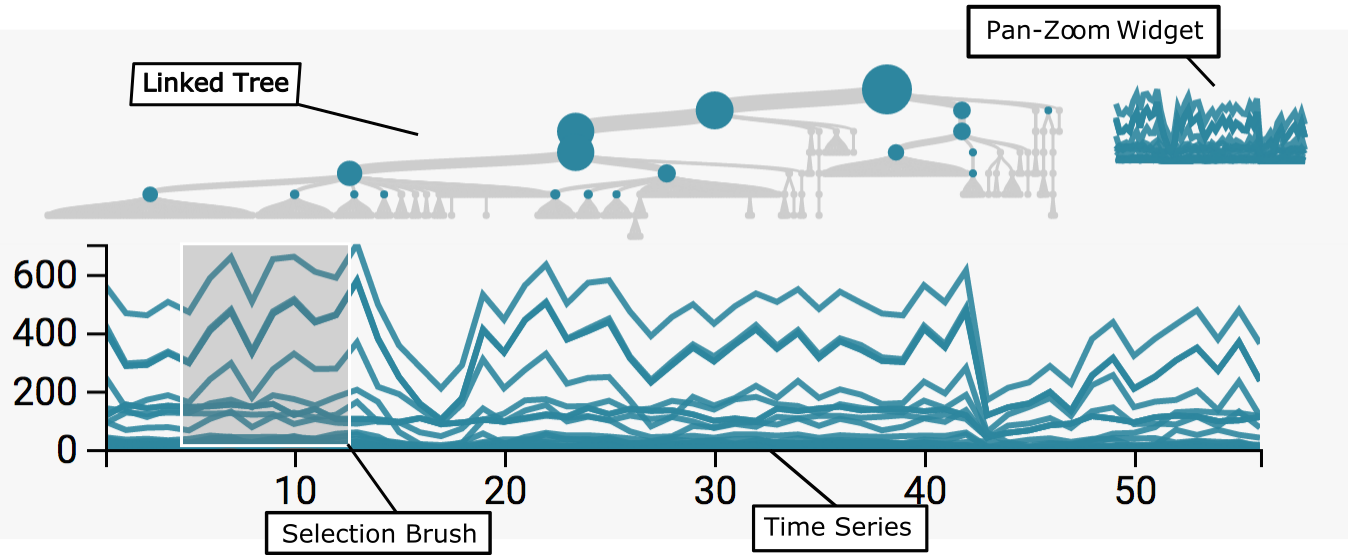
\includegraphics[width=350px]{figure/annotated_antibiotic_overview}

}

\caption{The two antibiotic time courses are readily apparent even when only highlighting the most abundant taxa. We have annotated the figure with its three main components.}\label{fig:antibioticoverview}
\end{figure}

\begin{figure}

{\centering 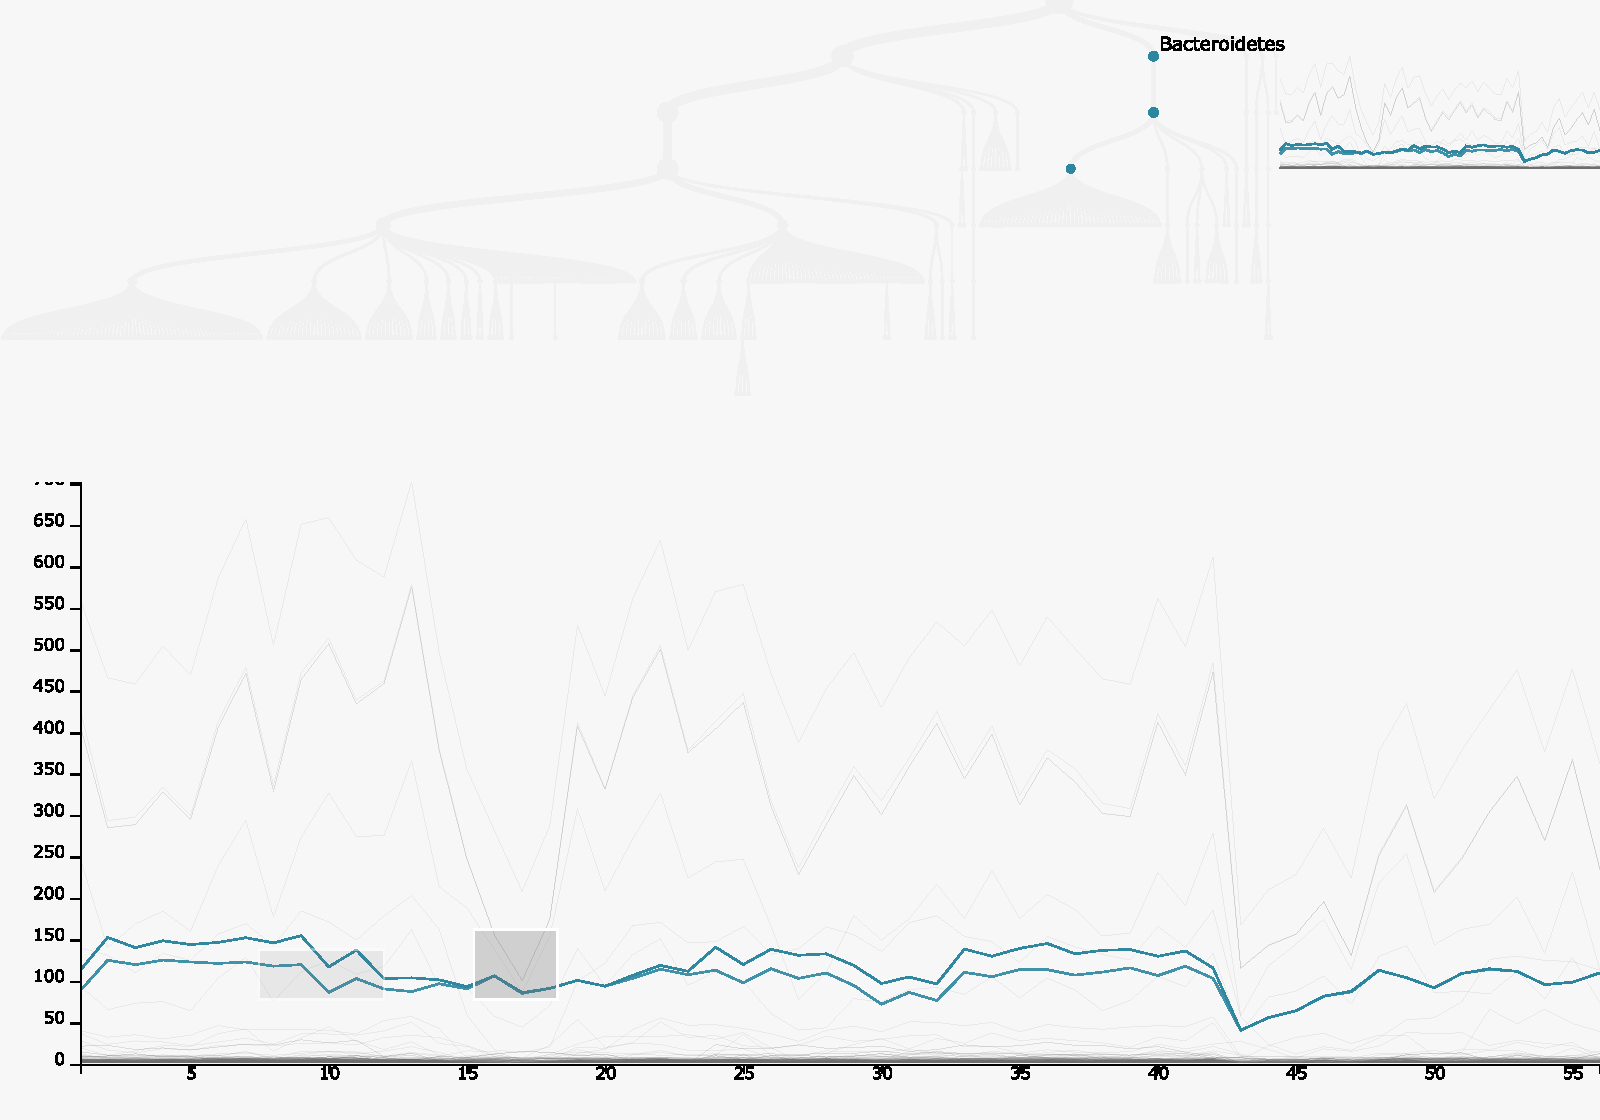
\includegraphics[width=350px]{figure/antibiotic_bacteroidetes}

}

\caption{Introducing a second box into the timebox display identifies the Bacteroidaceae as a taxon only midly impacted by antibiotics.}\label{fig:antibioticbacteroidetes}
\end{figure}

Next, using the scented widget, we focus on the window around the second
antibiotic treatment. We apply the treebox display to compare then
behavior of different families of Firmicutes, Lachnospiraceae and
Ruminoccocus. We suspect that these taxa are associated with the delayed
recovery after the second time course. To investigate this, we input
these family names in the search box to isolate their positions on the
tree; then we apply brushes to highlight the series that contribute to
these higher-level families. The resulting view is given by Figure
\ref{fig:antibioticfirmicutes}

\begin{figure}

{\centering 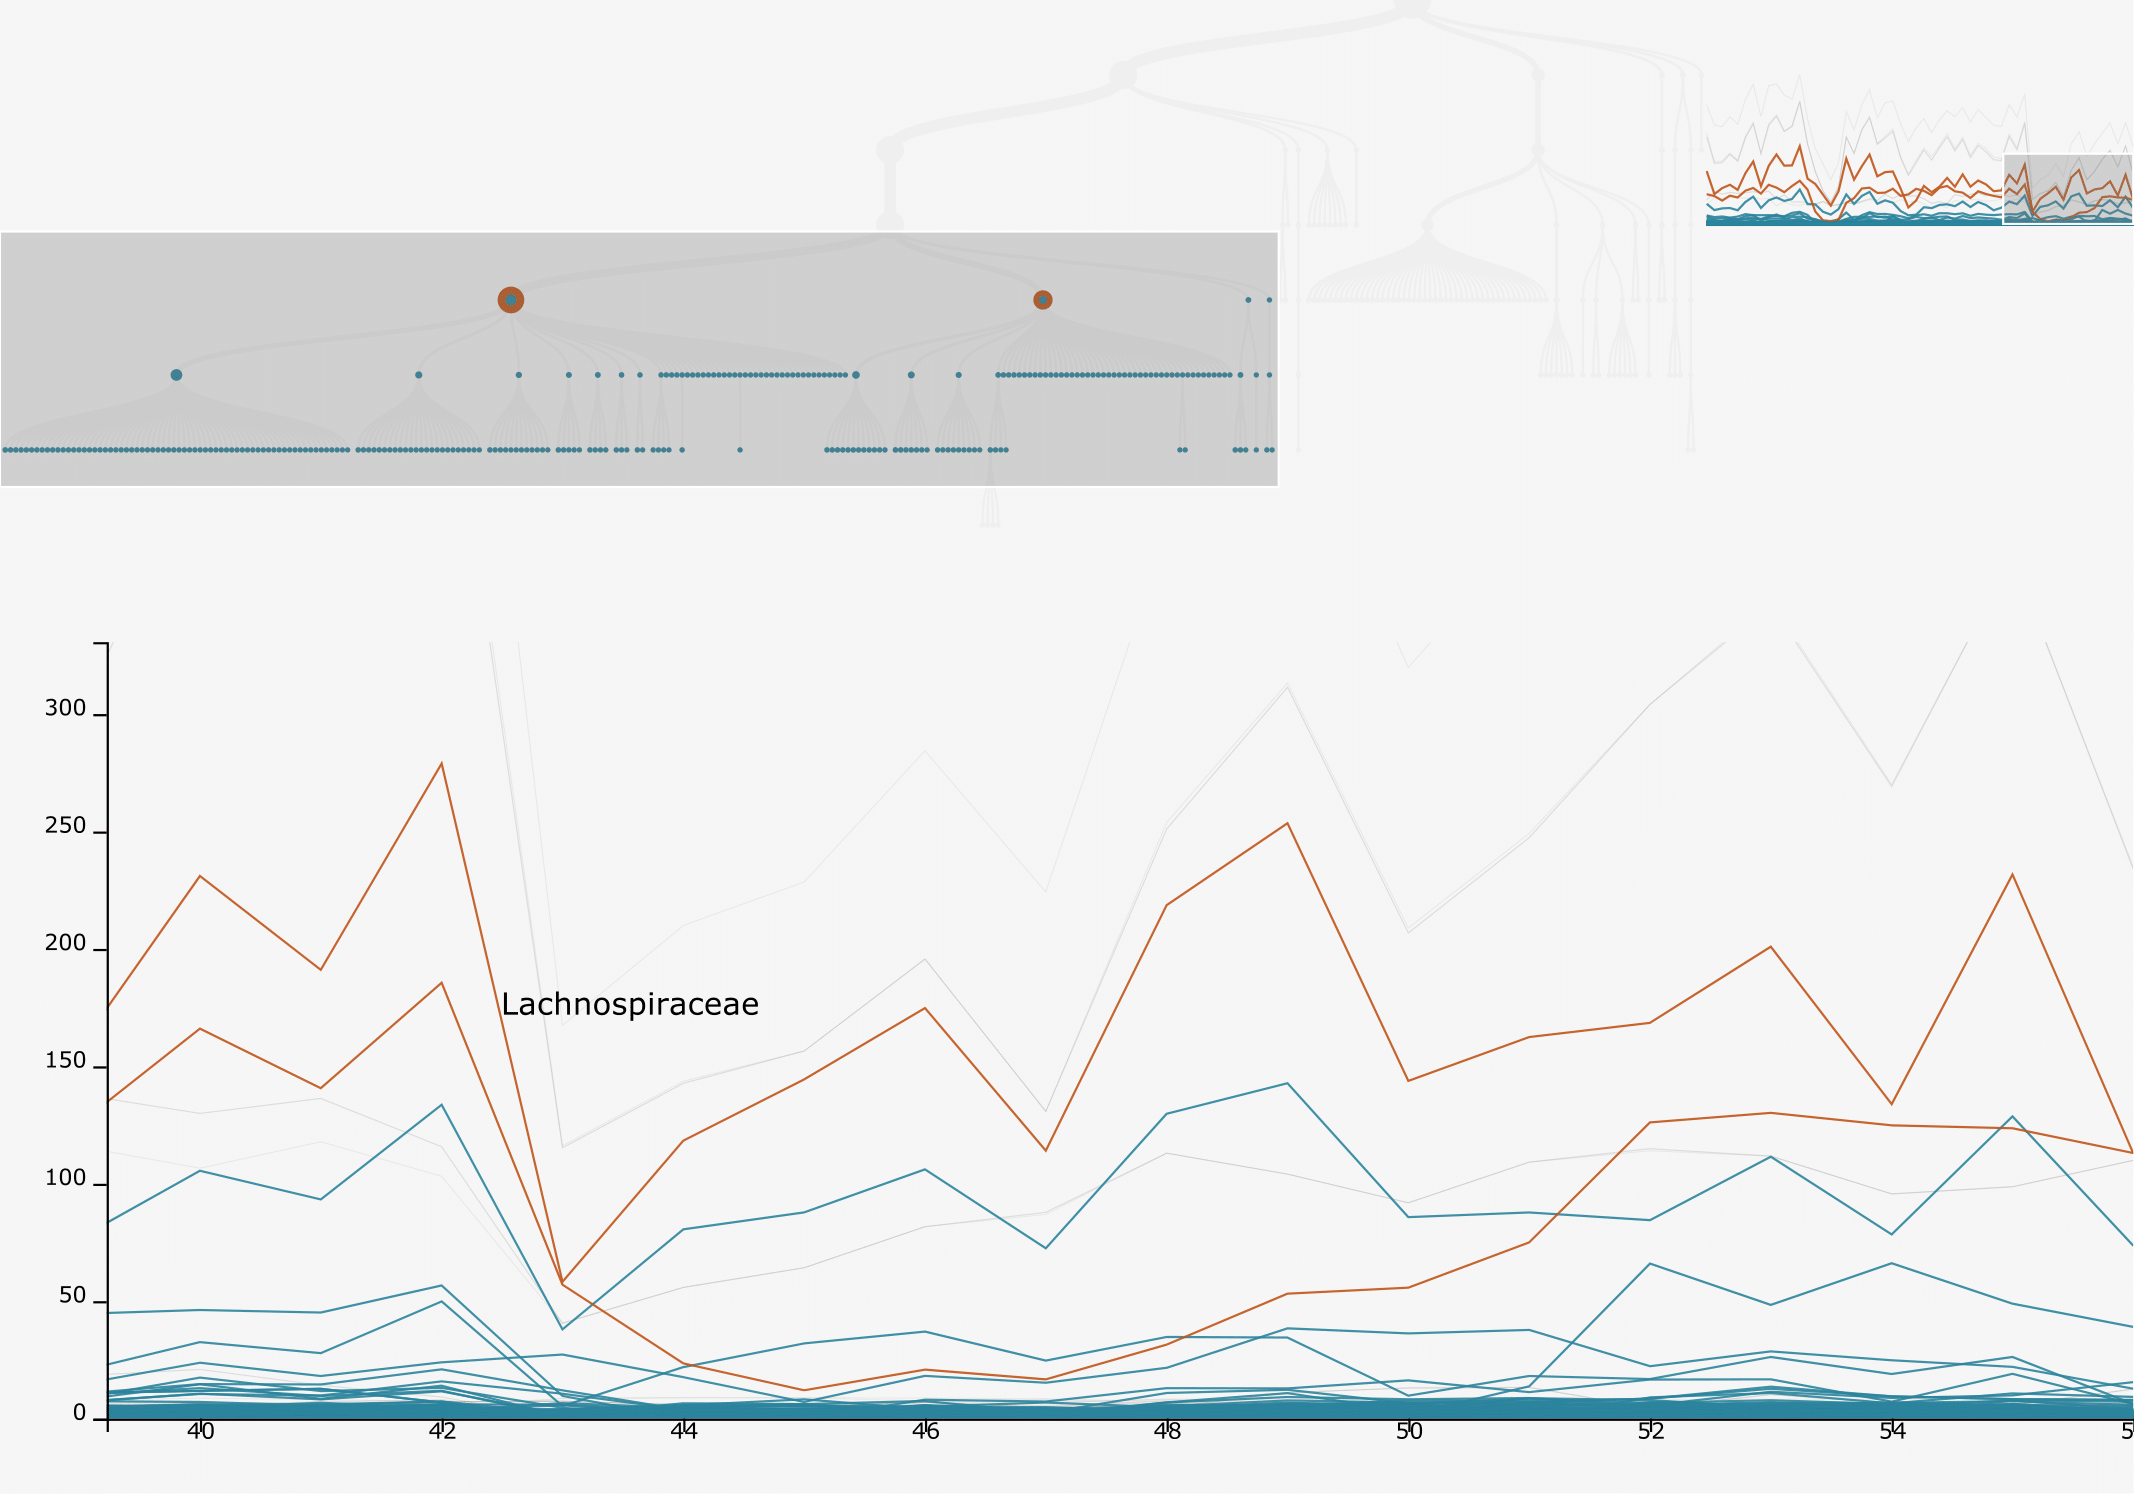
\includegraphics[width=350px]{figure/antibiotic_firmicutes}

}

\caption{Zooming into the second antibiotic timecourse and highlighting the Lachnospiraceae and Ruminococcus, we see that the Ruminoccocus took more time to recover to pre-treatment levels.}\label{fig:antibioticfirmicutes}
\end{figure}

Alternatively, we can summarize each node by the average across its
descendants -- this brings attention to individual bacteria that may be
underlying some of the broader taxonomic patterns we have noted when
studying the subtree sums. For example, in Figure
\ref{fig:ruminococcus}, we highlight all families below order
Ruminococcus, suggesting that the decrease due to antibiotics occurs
uniformly across almost all families. A point that was not evident in
the earlier sum-across-descendants view is that, after the second
treatment of antibiotics, a few of the Ruminoccocus families recover
more rapidly than the rest, for example the Unc095d3 (highlighted in
red) are only briefly affected. In contrast, most families seem to
recover in unison after the first treatment.

\begin{figure}

{\centering 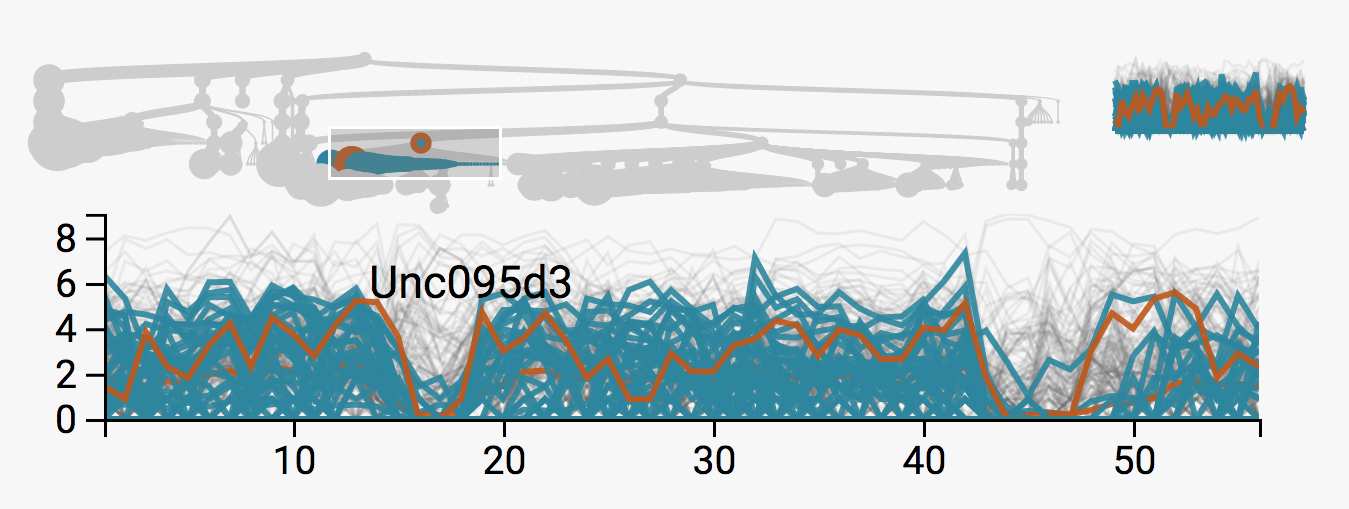
\includegraphics[width=350px]{figure/ruminococcus}

}

\caption{By hovering over the Ruminoccocus branches, we see that there is a prolonged effect of the antibiotics time courses more or less uniformly across the lower taxonomic orders.}\label{fig:ruminococcus}
\end{figure}

Further, note that in this subtree averages view, the tree display has
changed. This is because, at each branching point, we place the node
with larger average value on the left. This places the Verrucomicrobiae
at the far left, which seem to have large abundance over many time
points. This phylum had been previously obfuscated -- because there are
not many leaves associated with this phylum, the sum was small.
Interestingly, the abundance of these bacteria seems to \emph{increase}
after the first antibiotics treatment. Be cautious, however, that the
average over only a few Verrucomicrobiae species will be a more variable
estimate than the averages over the more prevalent phyla.

\begin{figure}

{\centering 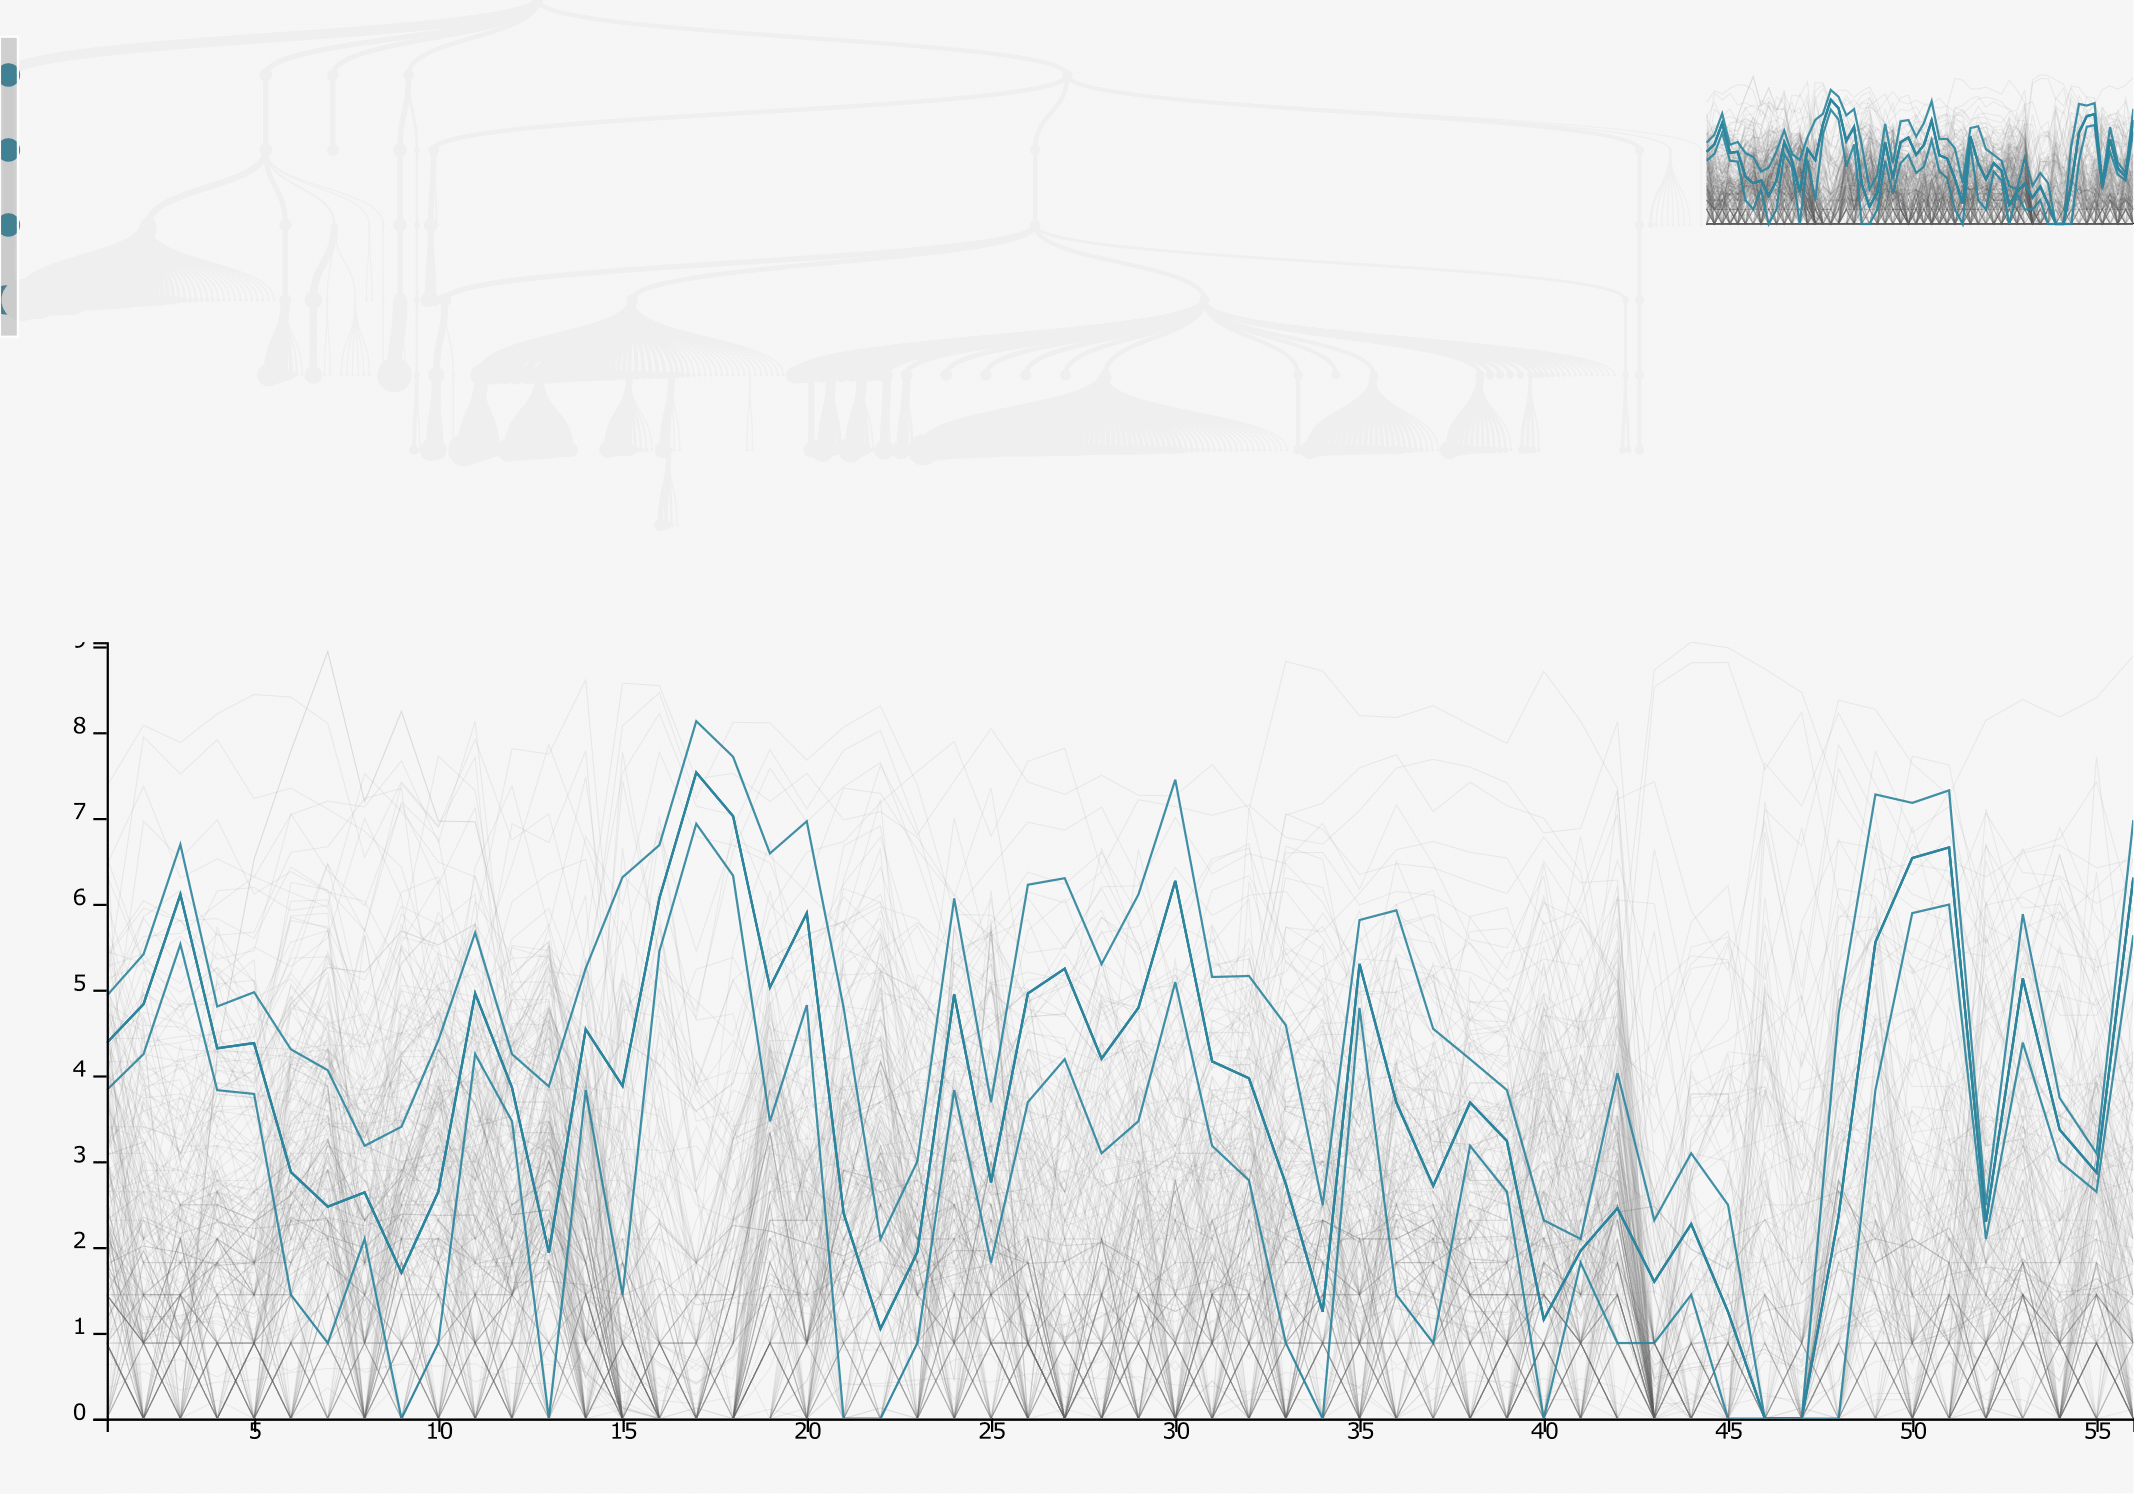
\includegraphics[width=350px]{figure/verrucomicrobiae}

}

\caption{The subtree averages aggregation brings attention to the Verrucomicrobiae, which though only present as a few species, are each rather abundant. In particular, they seem to increase after the first antibiotic time course.}\label{fig:verrucomicrobiae}
\end{figure}

\subsubsection*{Differential Bacterial Abundance and Preterm
Births}\label{differential-bacterial-abundance-and-preterm-births}

\citet{digiulio2015temporal}
tracked the abundance of bacteria in the vaginal microbiome during
pregnancy in an effort to study relationships between bacterial
community composition and preterm birth. Ideally, it would be possible
to develop clear bacterial signatures associated with preterm births.

Unlike the antibiotics study, we have measurements across more
individuals than we could reasonably inspect one at a time. While we
could average across all individuals, we will take our cue from
\citep{digiulio2015temporal}
place each sample into one of five Community State Types (CSTs),
identified via k-medoids. In that study, a linear model identified one
of these CSTs (CST 4) as significantly more diverse, further it appeared
associated with preterm births. Here, we corroborate this finding using
exploratory views.

Therefore, our focus here is on the differential abundance question,
rather than dynamics. We would like to provide visual representations of
differential abundance across CSTs and also between preterm and non-preterm
births. \citet{digiulio2015temporal} interpreted the CSTs using a heatmap, with
bacteria ordered according to a hierarchical clustering. By using the DOI sankey
instead, we can interpret the CSTs in their taxonomic context and at multiple
scales of taxonomic resolution. Further, while
\citet{digiulio2015temporal} focused on identifying associations between
preterm births and CSTs -- presumably because testing individual bacteria loses
power -- we can compare bacterial abundances between preterm and non-preterm
samples along subtrees, without requiring CSTs as an intermediary.

In Figure \ref{fig:pretermcsts}, we compare the 5 CSTs according to
their values along the subtree. Specifically, we took the average of all
samples within each CST to define values at the (species-level) leaf
nodes, and then aggregated the averages up to the root. It is
immediately clear that samples from CST 4 have much more taxonomic
diversity. Further, focusing on the Lactobacillaceae family, we note
that the differential abundance of these bacteria distinguishes the
remaining CSTs, see Figure \ref{fig:pretermcstslacto}.

Alternatively, in Figure \ref{fig:pretermpreterm}, we avoid working with
CSTs, displaying instead averages among samples associated with either
preterm or term births. The red edges are associated with preterm
births -- we see that they contribute more weight to phyla outside the
Firmicutes. This is consistent with the claim that CST 4, the most
diverse of the CSTs, is associated with preterm births.

\begin{figure}

{\centering 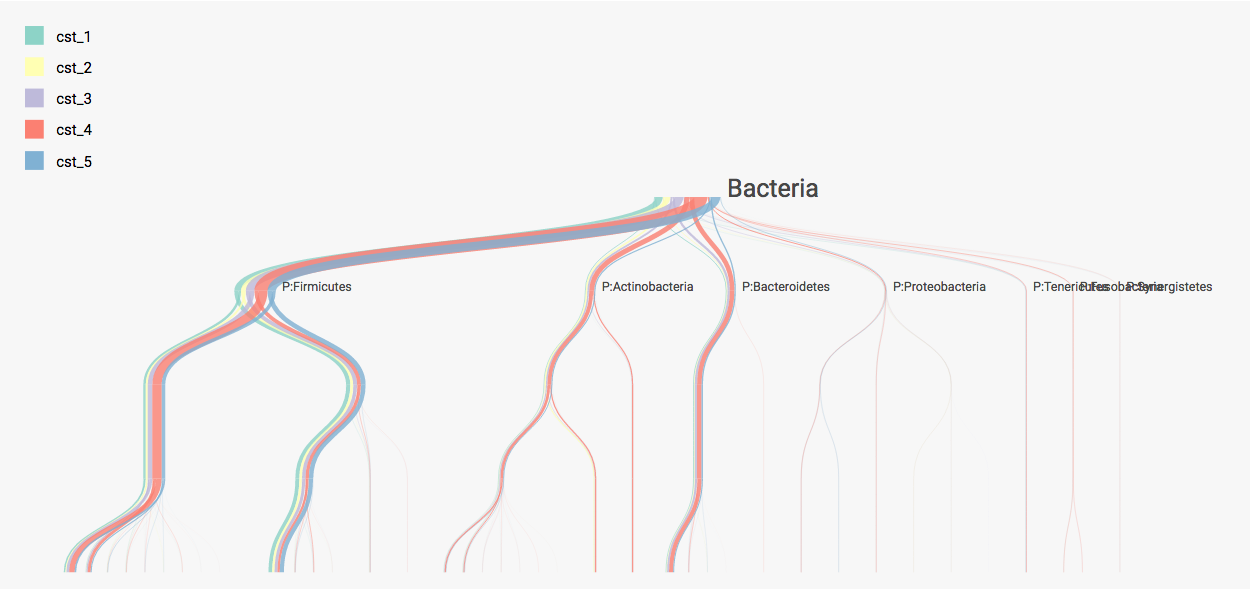
\includegraphics[width=350px]{figure/preterm_csts}

}

\caption{The increased diversity among samples in CST 4 is represented by the relatively larger contribution of red edges to branches outside of the Firmicutes.}\label{fig:pretermcsts}
\end{figure}

\begin{figure}

{\centering 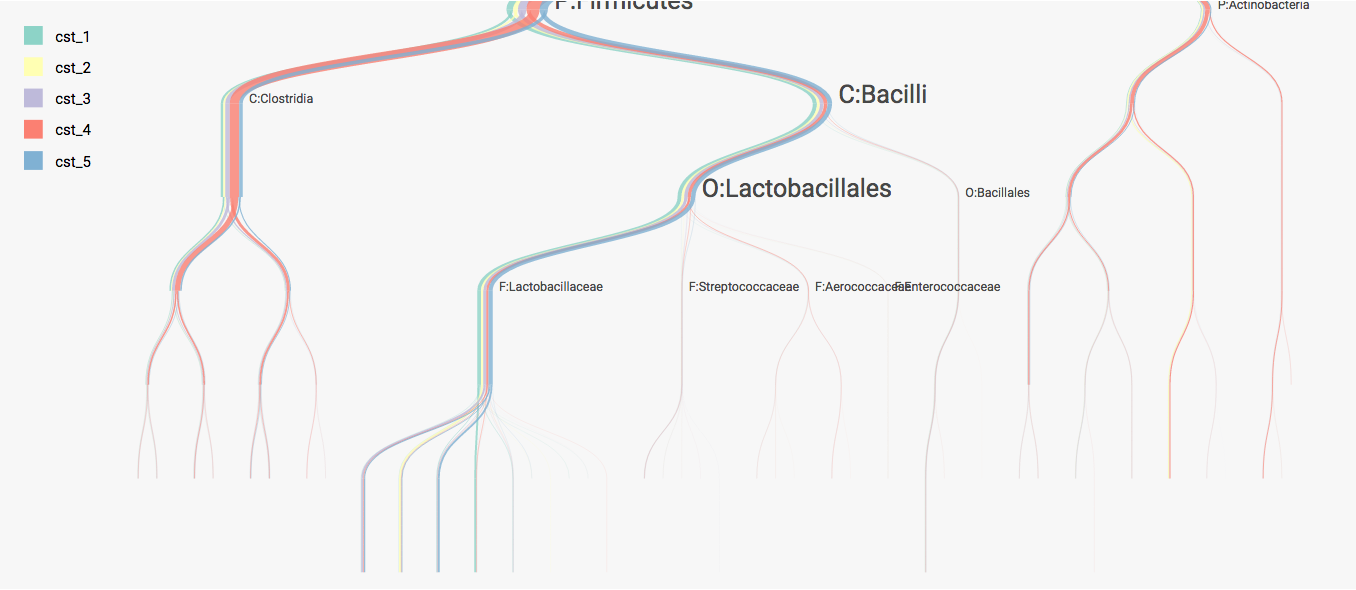
\includegraphics[width=350px]{figure/preterm_csts_lacto}

}

\caption{Zooming into the Lactobacillaceae family, we notice that the difference between the remaining four CSTs is related to which types of Lactobacillus are most prominent.}\label{fig:pretermcstslacto}
\end{figure}

\begin{figure}

{\centering 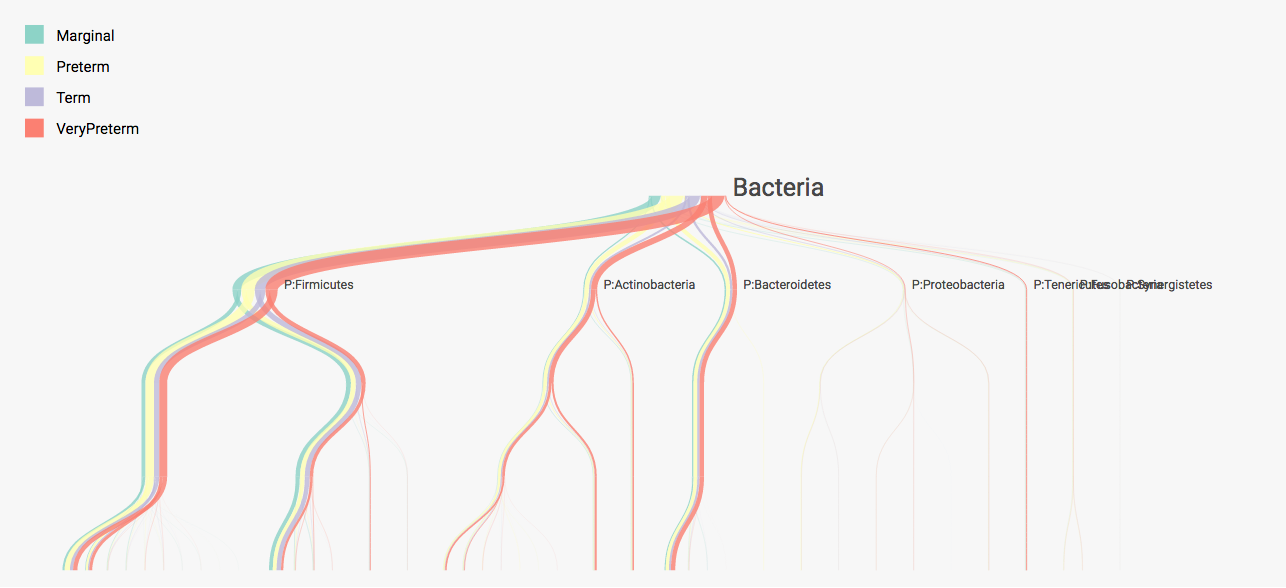
\includegraphics[width=300px]{figure/preterm_preterm}

}

\caption{Samples with high levels of phyla other than Firmicutes appear to be related to preterm births.}\label{fig:pretermpreterm}
\end{figure}

\subsubsection*{Dynamics in Housing Prices}\label{zillow-study}

We next consider an application unrelated to the microbiome, but with
relatively clear hierarchical structure. Our data are downloaded from
Zillow\footnote{\url{http://www.zillow.com/research/data/}}, and give
the Zillow Home Value Indexes at the neighborhood level, across the
country, computed monthly between 1996 and 2016. In our display, we have
taken the base 10 log of these indexes. As our hierarchical structure,
we use each neighborhood's assignment to state, regional, county, and
city levels. We represent each of these coarser spatial categories using
the average of all neighborhoods contained in them. We have filtered
down to the 890 neighborhoods in California; rendering more
neighborhoods while keeping all 246 timepoints causes the interface to
lag\footnote{See below for potential optimizations, however.}.

Our basic analysis revolves around geographic and temporal variation in
home prices. We are especially interested in the effect of the 2008
recession and any variation in the lead-up to or recovery from this
event. These questions can be naturally framed using timebox trees and
treeboxes.

We first study variation in prices at the city level. These series can
be highlighted using a single brush in treeboxes, since each spatial
level is displayed at the same height in the tree. The resulting display
is given in Figure \ref{fig:zillowcities}. From a high level, the
housing bubble, decrease in prices due to the recession, and subsequent
recovery are readily apparent. The city-level view makes it clear that
not all neighborhoods were equally affected by the recession -- richer
cities plateaued at their 2008 prices, middle-income cities saw moderate
decreases, and poorer cities saw the most significant declines in home
prices. These more significant declines tended to occur in cities that
had recently seen rapid increases during the housing bubble. Finally, we
note that the range in home prices seems to have increased after the
recession, speaking to the differential long-term effect of the
recession on prices.

Alternatively, we can study the trajectories of home prices among
neighborhoods, conditional on their being middle-income before the
recession. We generate the sequence of views in Figures
\ref{fig:zillowmiddlepre}, \ref{fig:zillowmiddleup}, and
\ref{fig:zillowmiddledown} to this end. The first of these figures
isolates neighborhoods with middle incomes before the recession, using a
single timebox. Since there appears to be a divergence in trajectories
after the recession, we introduce a second post-recession timebox,
dragging it over series with higher and lower incomes during this second
time period. This is the content of Figures \ref{fig:zillowmiddleup} and
\ref{fig:zillowmiddledown}. Inspecting the highlighted tree nodes
associated with these series, we find that most of the middle-income
series that increased after the recession are associated with
middle-income neighborhoods within the coastal Southern California
counties. In constrast, those middle income series that saw decreases
were mostly located in Central California and Oakland.

The previous analysis highlights the fact that, within even narrow
geographic regions, there can be substantial variation in prices. We can
study this directly using treeboxes. In Figure \ref{fig:zillowsf} we
have highlighted all series in San Francisco County. We see that, in
2016, prices range from around \(10^{5.6} \approx \$400,000\) to
\(10^{6.7} \approx \$5 \text{ million}\). So, while all these
neighborhoods tend to be among the more expensive ones in California,
prices can vary in a non-smooth way across geographic space.

We conclude this example with a caveat that the Zillow data are not
representative of all neighborhoods in California, only those with
enough listings on the site, so should be supplemented by other data
sources for any substantial decision-making.

\begin{figure}

{\centering 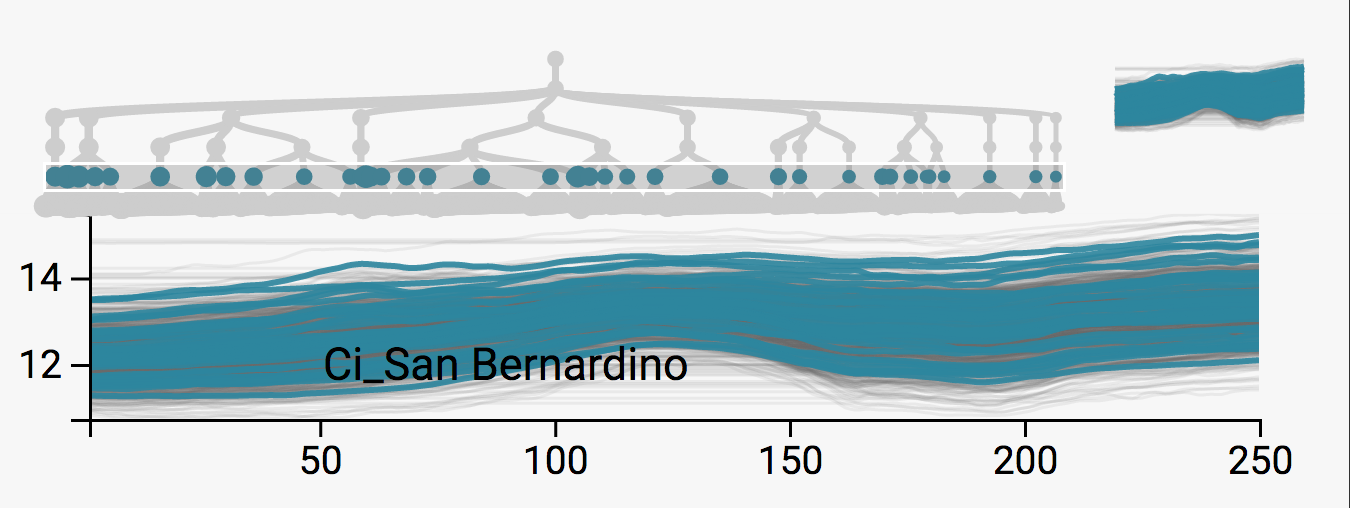
\includegraphics[width=350px]{figure/zillow_cities}

}

\caption{California home prices at the city level, between 1996 and 2016. The effect of the 2008 recession is clear, and we have hovered over the San Bernardino series, to display the identity of one of the cities most strongly affected by the recession.}\label{fig:zillowcities}
\end{figure}

\begin{figure}

{\centering 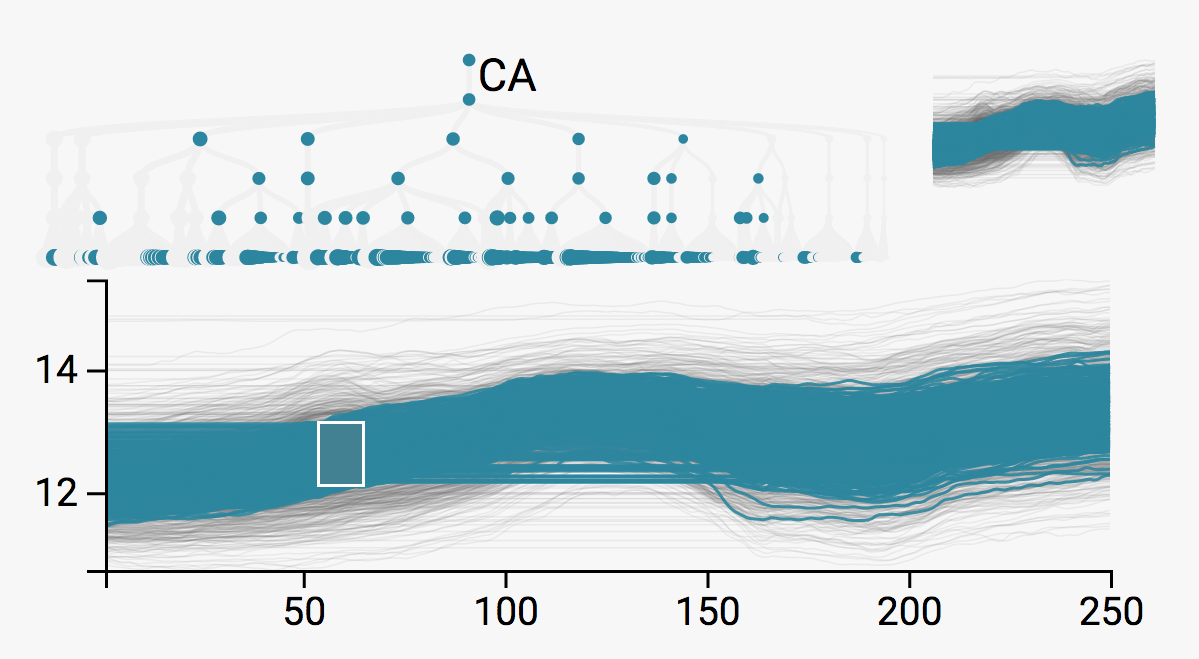
\includegraphics[width=350px]{figure/zillow_middle_pre}

}

\caption{Neighborhoods with mid-range home prices before the recession are selected here. Note that the collection of series seems to widen after 2008 -- we are interested in whether there are reliable predictors of these alternate trajectories, given their similar starting points.}\label{fig:zillowmiddlepre}
\end{figure}

\begin{figure}

{\centering 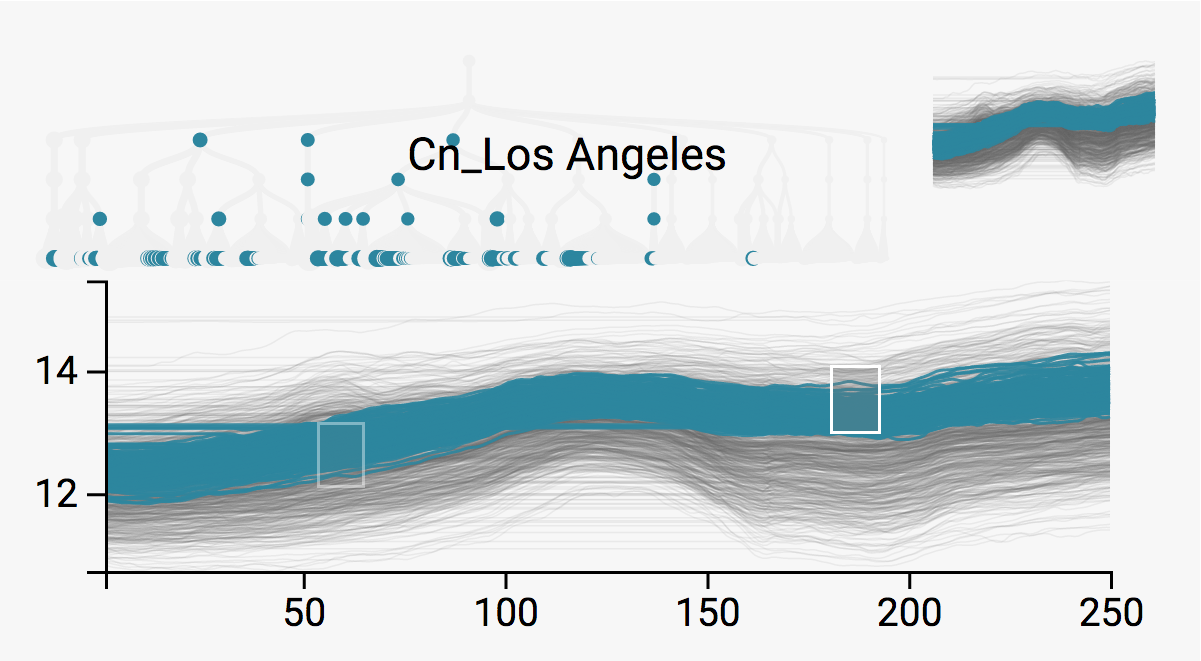
\includegraphics[width=350px]{figure/zillow_middle_up}

}

\caption{Among those neighborhoods with mid-range prices before the recession, we have selected those that recovered more rapidly. These appear to be located mainly in Los Angeles and San Diego counties.}\label{fig:zillowmiddleup}
\end{figure}

\begin{figure}

{\centering 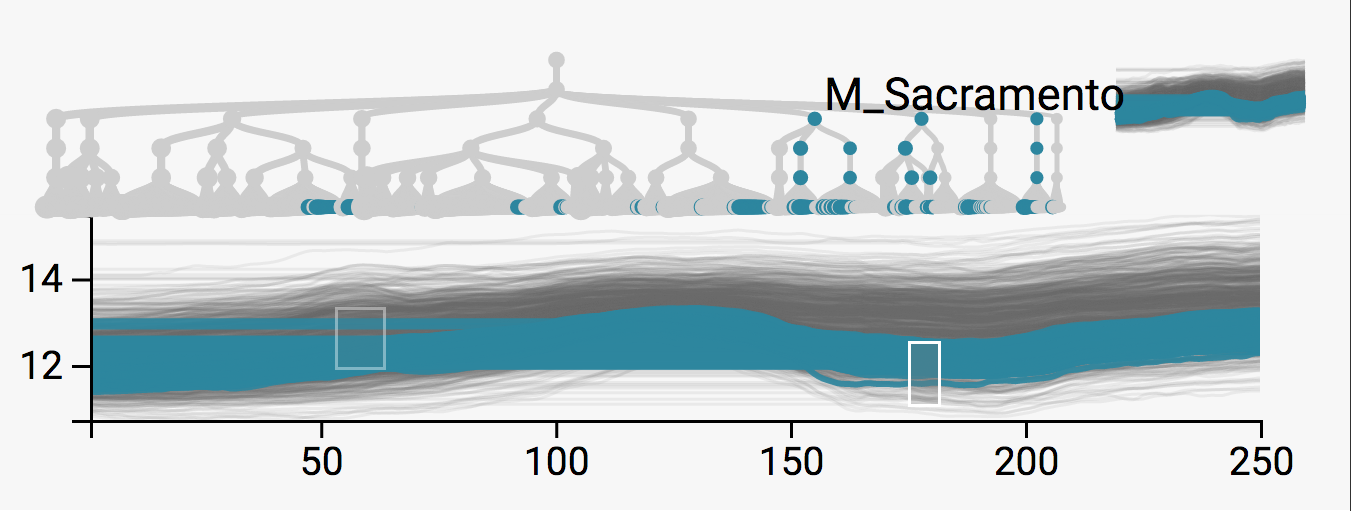
\includegraphics[width=350px]{figure/zillow_middle_down}

}

\caption{Rather than selecting mid-range series that recovered quickly, we can isolate those whose prices remained depressed after the recession. These seem mostly to be located in Central California and the East San Francisco Bay Area.}\label{fig:zillowmiddledown}
\end{figure}

\begin{figure}

{\centering 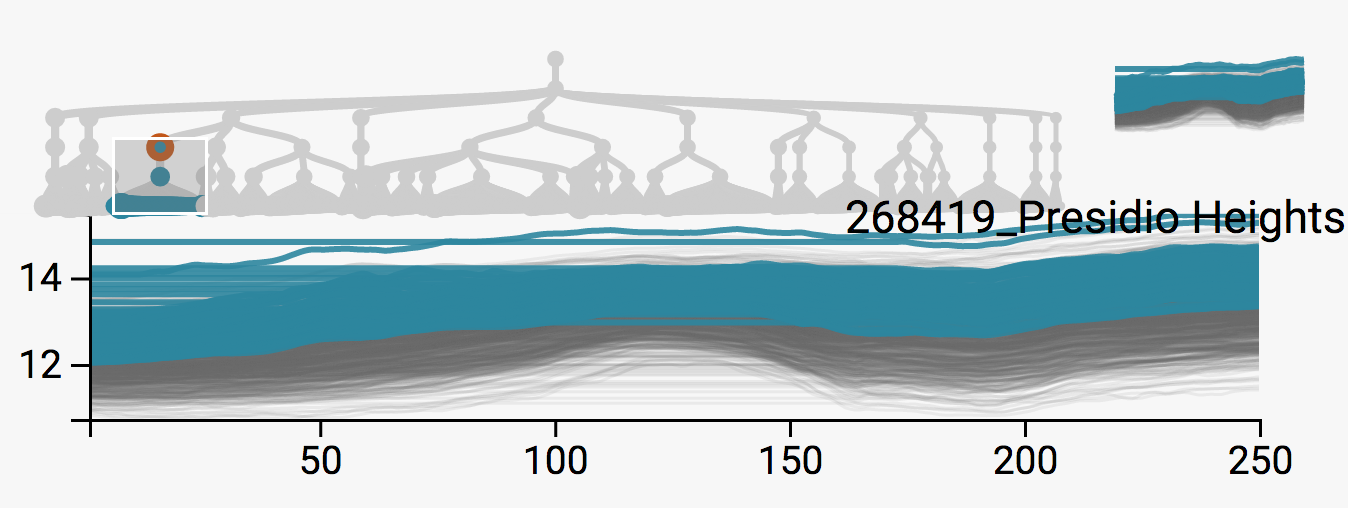
\includegraphics[width=350px]{figure/zillow_sf}

}

\caption{To study the range in home prices within San Francisco County, we can select the associated nodes using a treebox.}\label{fig:zillowsf}
\end{figure}

\subsubsection*{Sources of Variation in Bikesharing
Demand}\label{bikesharing-study}

Our next example is a study in bikesharing demand, included as an
example of analyzing collections of time series when there is no obvious
hierarchical structure a priori. The data are available at the UCI
Repository\footnote{\url{https://archive.ics.uci.edu/ml/datasets/Bike+Sharing+Dataset}}
and were originally collected by a Washington D.C.-based bikesharing
system for use in a Kaggle prediction competition. The data are hourly
measurements of bike demand, aggregated across all bikesharing stations,
over two years, along with supplemental weather data. In the
competition, participants were asked to predict the hourly demand on a
held-out test set. Here, we adopt a descriptive view instead, attempting
to characterize factors associated with variation in bikesharing demand.

Like the Zillow home prices application, we study this problem as one of
describing a large collection of related time series. Here, we consider
the demand during a single day to be one time series; this is a natural
choice considering the daily periodicity of bike demand. To arrange
these daily series along an interpretable tree structure, we apply a
regression tree relating the supplemental data to the bikesharing demand
\citep{breiman1984classification}. In more
detail, we built this tree by noting the ``two table'' structure of this
problem: one describes bike demand, the other holds the supplemental
data. In both, the rows index days, while the columns index either hours
or supplemental features. Our tree is the trained regression tree after
predicting demand at 8AM based on the supplemental data. We choose this
response because (1) we need a univariate response in order to apply
regression trees and (2) the more straightforwards reduction to
daily-average-demand fails to distinguish between weekdays and weekends,
whose series appear qualitatively very different from each other.

Given this response, the first split in the regression tree is
(unsurprisingly) the difference between weekends and weekdays. This is
emphasized in Figures \ref{fig:working} and \ref{fig:weekend}, respectively;
using timeboxes to isolate the two types of series highlight the left and right
sides of the tree, respectively. For a more subtle effect, we select the
internal nodes associated with the first split below the weekday vs. weekend
split; these are given in Figures \ref{fig:weekday2011} and
\ref{fig:weekday2012}. This suggests that weekday demand increased during the
second year.

\begin{figure}

{\centering 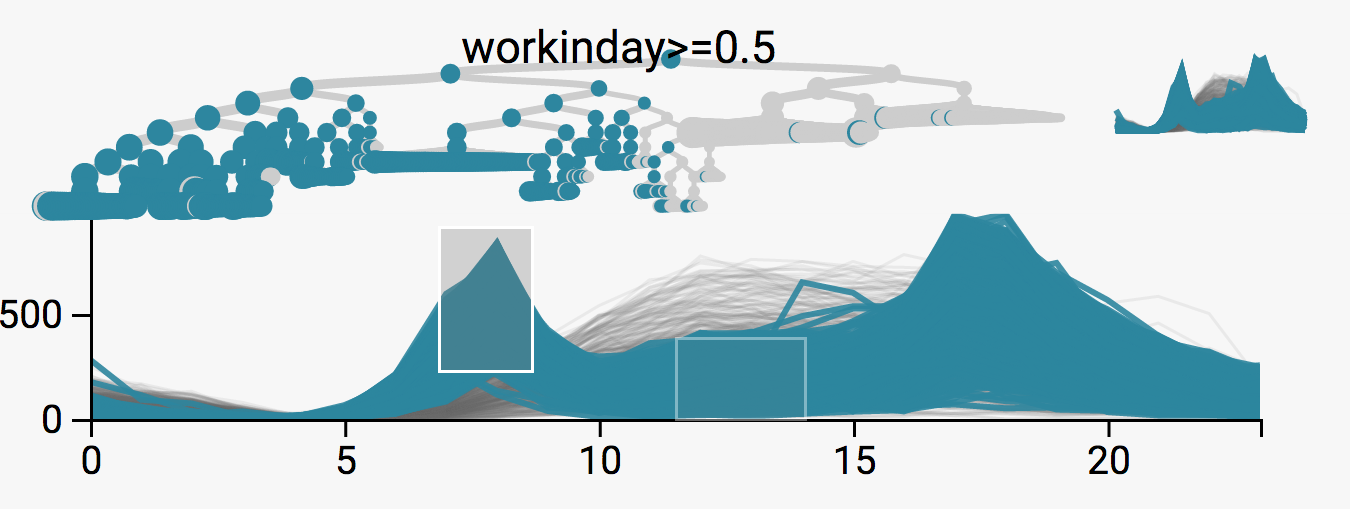
\includegraphics[width=350px]{figure/working}

}

\caption{The two peaks at rush hour distinguish weekday series from the rest.}\label{fig:working}
\end{figure}

\begin{figure}

{\centering 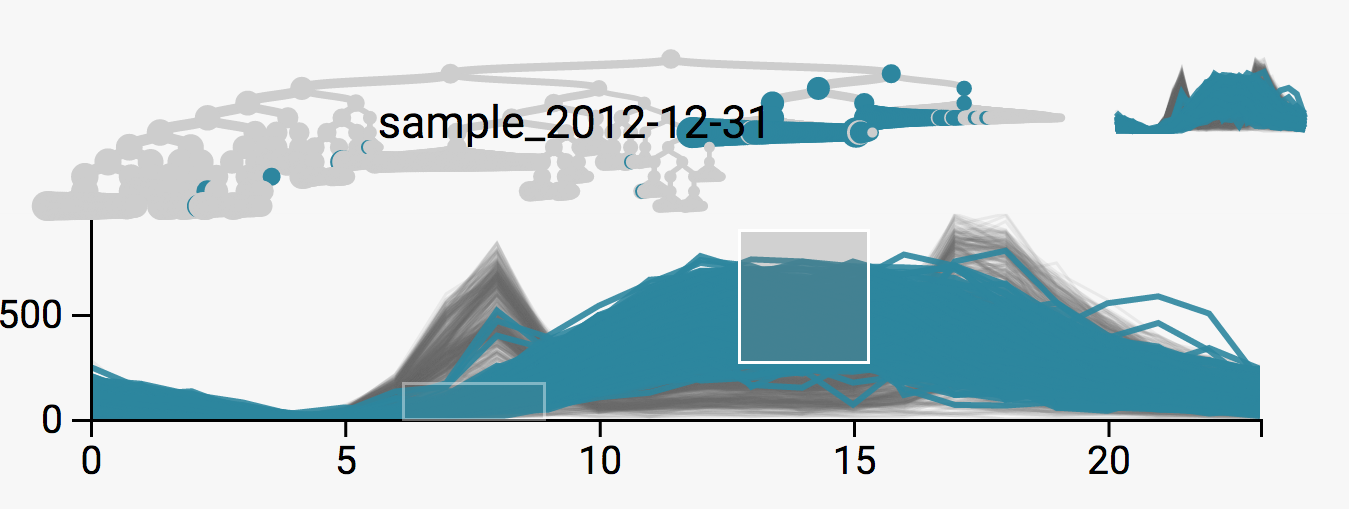
\includegraphics[width=350px]{figure/weekend}

}

\caption{Unlike weekday demand, weekend demand is unimodal. The few weekday series with unimodal series seem to be associated with holidays. This is the case for New Years' Eve, which is currently hovered over in the tree.}\label{fig:weekend}
\end{figure}

\begin{figure}

{\centering 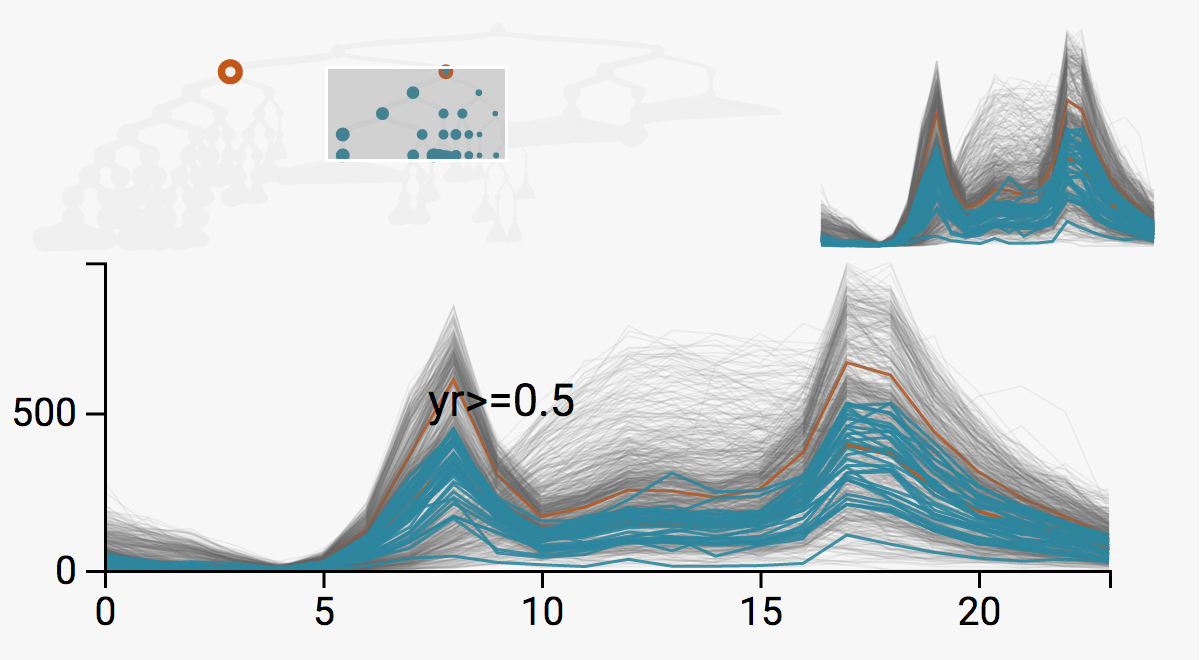
\includegraphics[width=350px]{figure/weekday_2011}

}

\caption{Weeday demand appears larger in 2012 than 2011 -- compare with the next figure.}\label{fig:weekday2011}
\end{figure}

\begin{figure}

{\centering 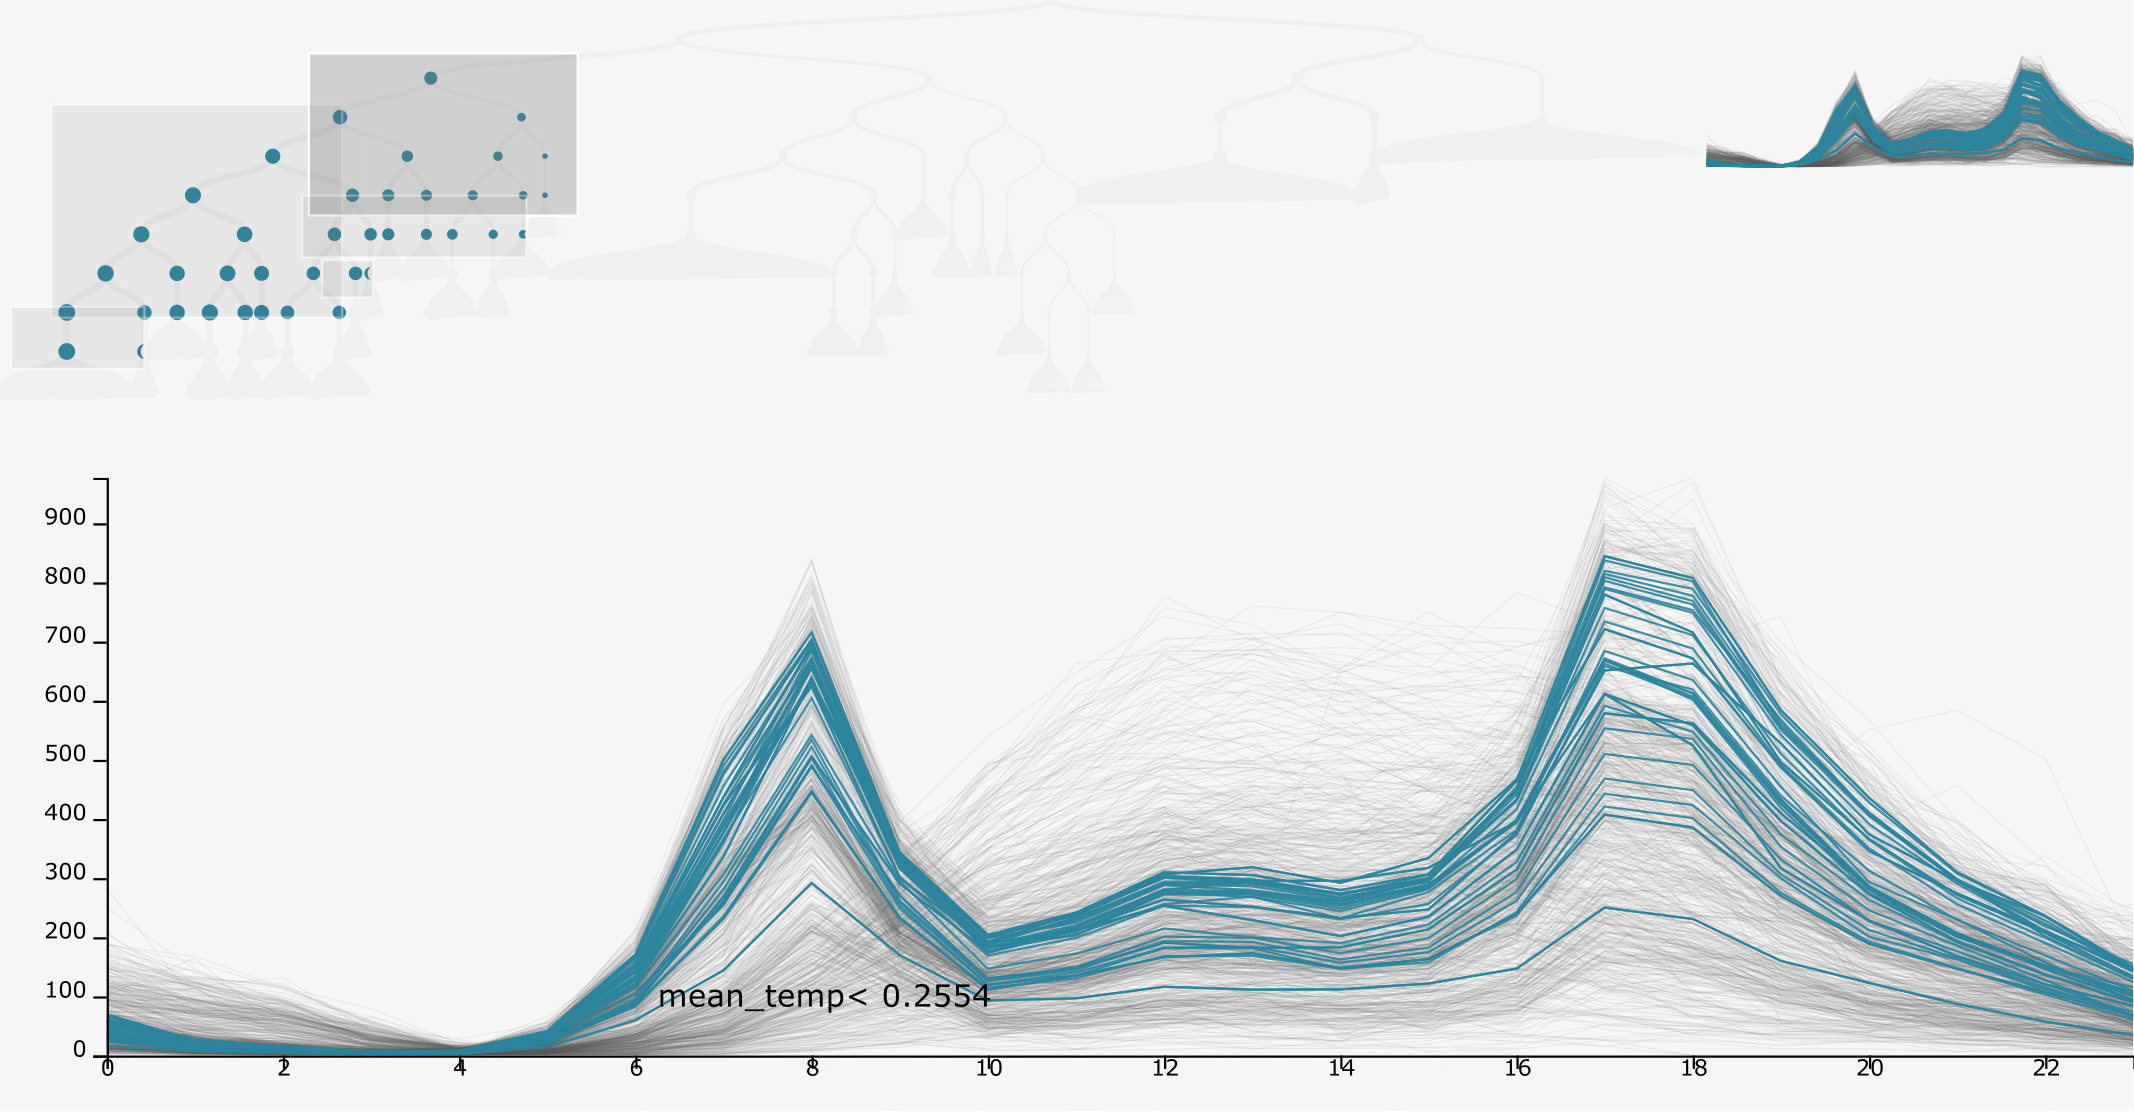
\includegraphics[width=350px]{figure/weekday_2012}

}

\caption{Weekday demand increased in 2012 -- compare with the previous figure.}\label{fig:weekday2012}
\end{figure}

In contrast to these general questions about daily demand, we could ask
a more granular question about specific time windows. For example, what
characterizes days on which there is larger than average demand after
midnight? We can select these series after first zooming into this time window.
Figure \ref{fig:warmweekend} reveals that the highlighted series are associated
with the warm-weekend split, which seems quite reasonable in retrospect.

\begin{figure}

{\centering 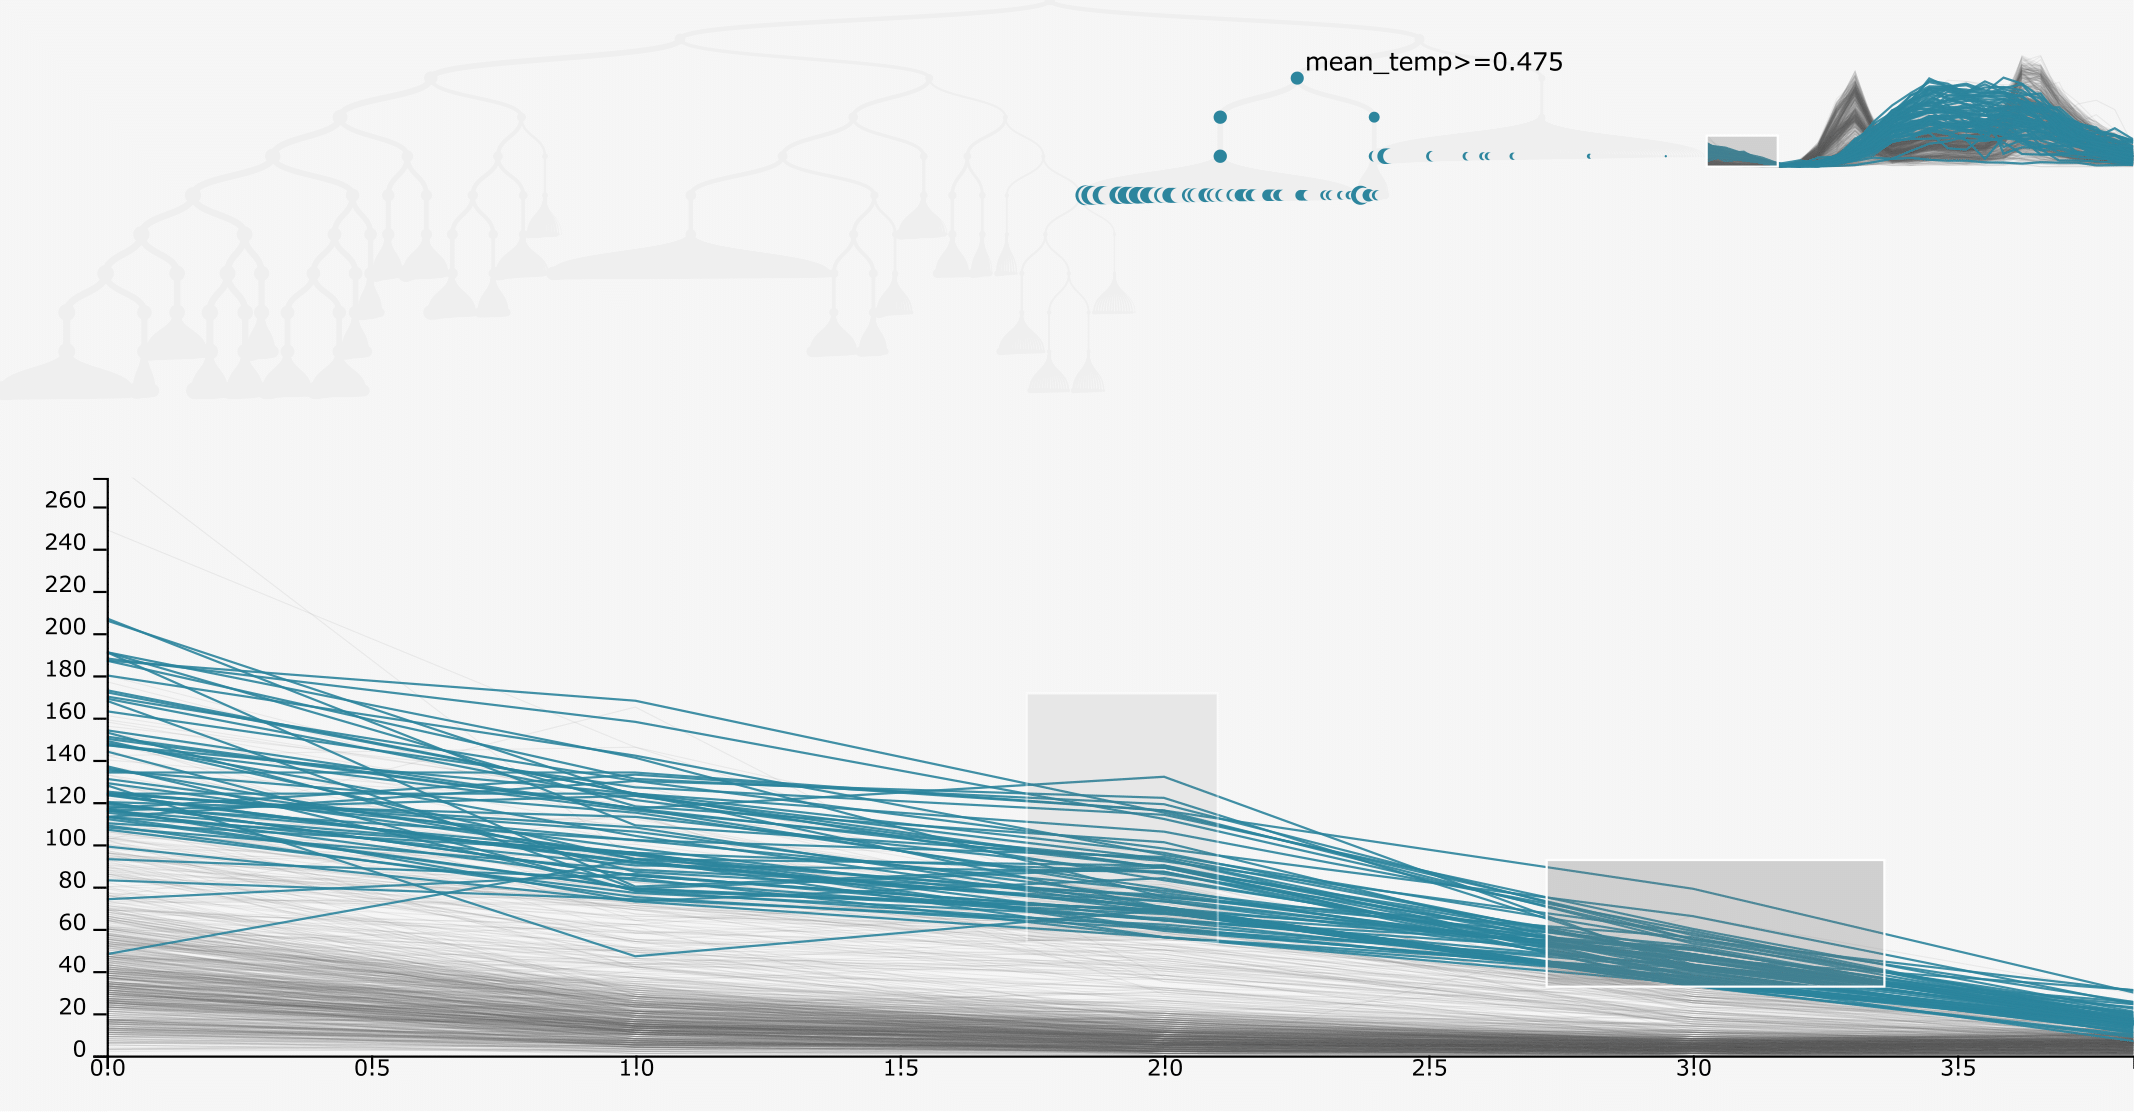
\includegraphics[width=350px]{figure/warm_weekend}

}

\caption{The samples with highest night demand tend to fall on warm weekends.}\label{fig:warmweekend}
\end{figure}

Finally, we can study the behavior of the regression tree itself using
the DOI sankey. Here, we group samples according to their quintile of
8AM demand and then count the abundance of the groups flowing down
different branches. We find that the quintiles are each rather strongly
separated after descending even a few steps down the regression tree --
for example, Figures \ref{fig:weekday2011} and \ref{fig:weekday2012}
focus on 2011 vs. 2012 split among weekday samples, showing that this
split distinguishes between samples falling in the second and third
quintiles of 8AM demand.

\begin{figure}

{\centering 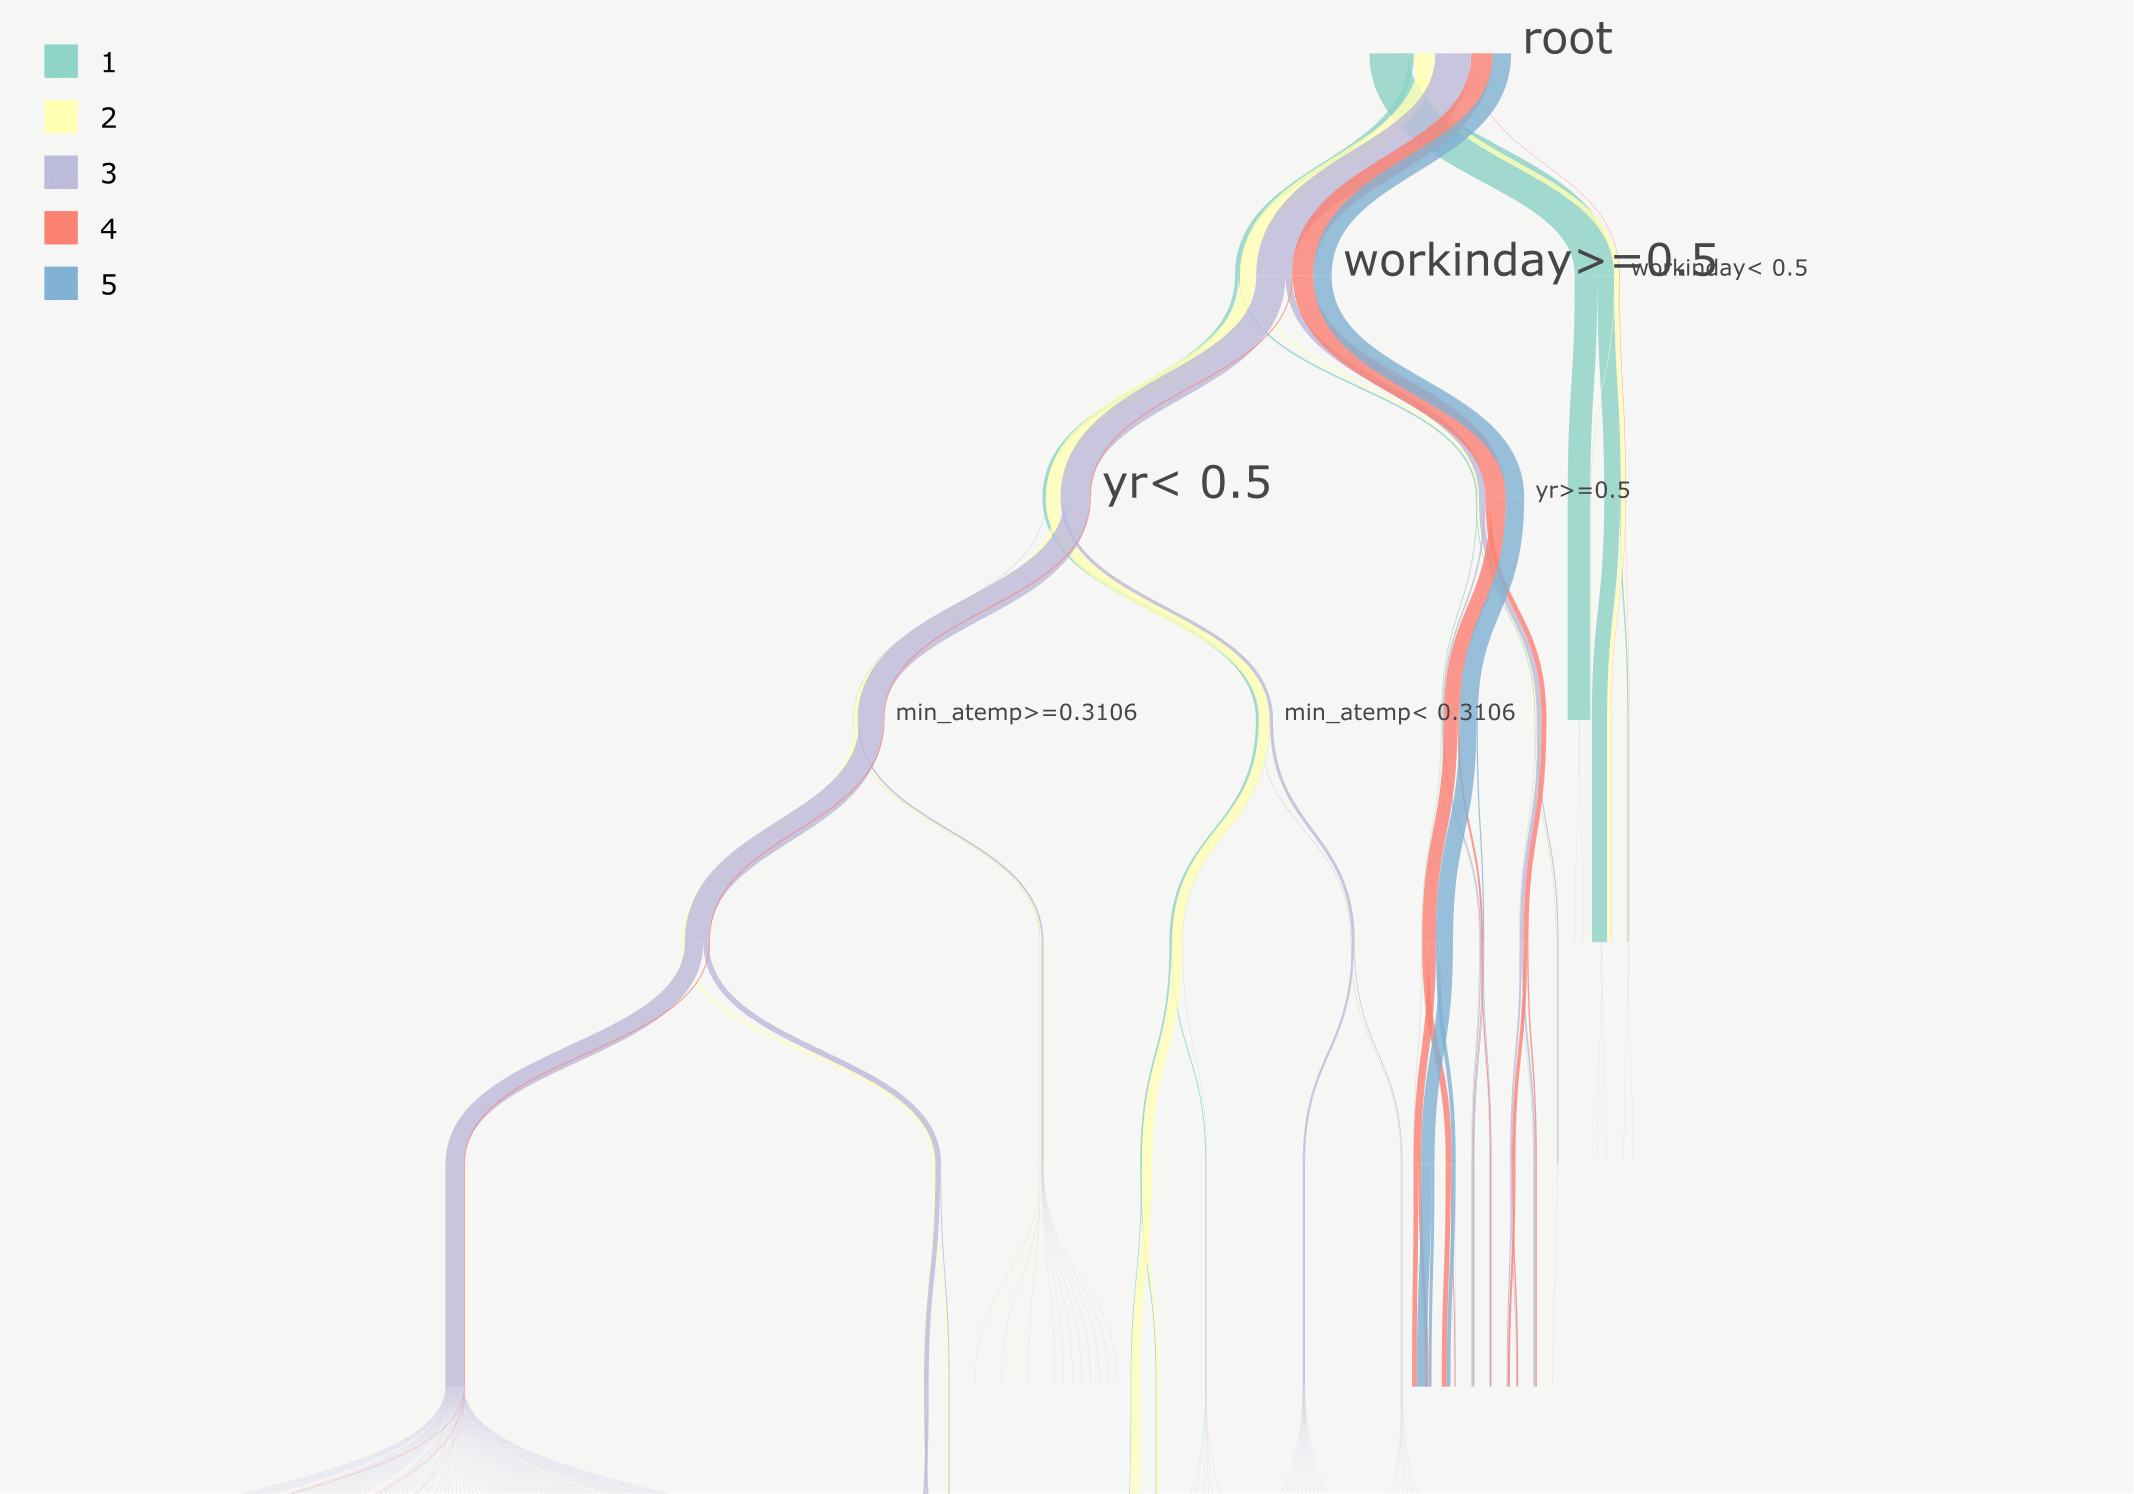
\includegraphics[width=350px]{figure/bike_sankey}

}

\caption{We can interpret the regression tree using an interactive DOI representation.}\label{fig:bikesankey}
\end{figure}

This interactive representation of regression trees is potentially more
useful on larger trees that cannot be easily parsed in a single view; in
this sense the bikesharing tree is relatively simple. In our ideal data
analysis workflow, we imagine the analyst applying interactive
visualization and modeling techniques in an iterative, nonlinear
fashion.

\subsubsection*{Hierarchically Clustering the Global Patterns Data}\label{global_patterns}

Each of the timebox tree and treebox examples presented so far have
focused on data with a clear time component. We note however that these
techniques could alternatively be applied to high-dimensional data, via
the use of parallel coordinates \citep{inselberg1991parallel}. The usual
parallel coordinates challenges remain, namely selecting scales for and an
ordering across the different coordinates, but the linking and
focus-plus-context ideas can still be employed in this setting. Here we
provide an implementation of this idea on a dataset comparing microbiomes across
various ecological environments \citep{caporaso2011global}, which is publicly
accessible through the phyloseq R package \citep{mcmurdie2013phyloseq}.

The original Global Patterns data consists of 26 samples across 9
environments (for example, freshwater and soil). In each site, there are
counts across 19216 taxa -- to simplify visualization, we filter to the
500 most abundant taxa.

We hierarchically cluster these 26 samples based on the 500 most
abundant taxa, using complete linkage on the UniFrac distance. Figure
\ref{fig:gptimebox} displays the resulting hierarchy together with a
parallel coordinates view of the \(\text{asinh}\) transformed taxa.

\begin{figure}
  {
    \centering
    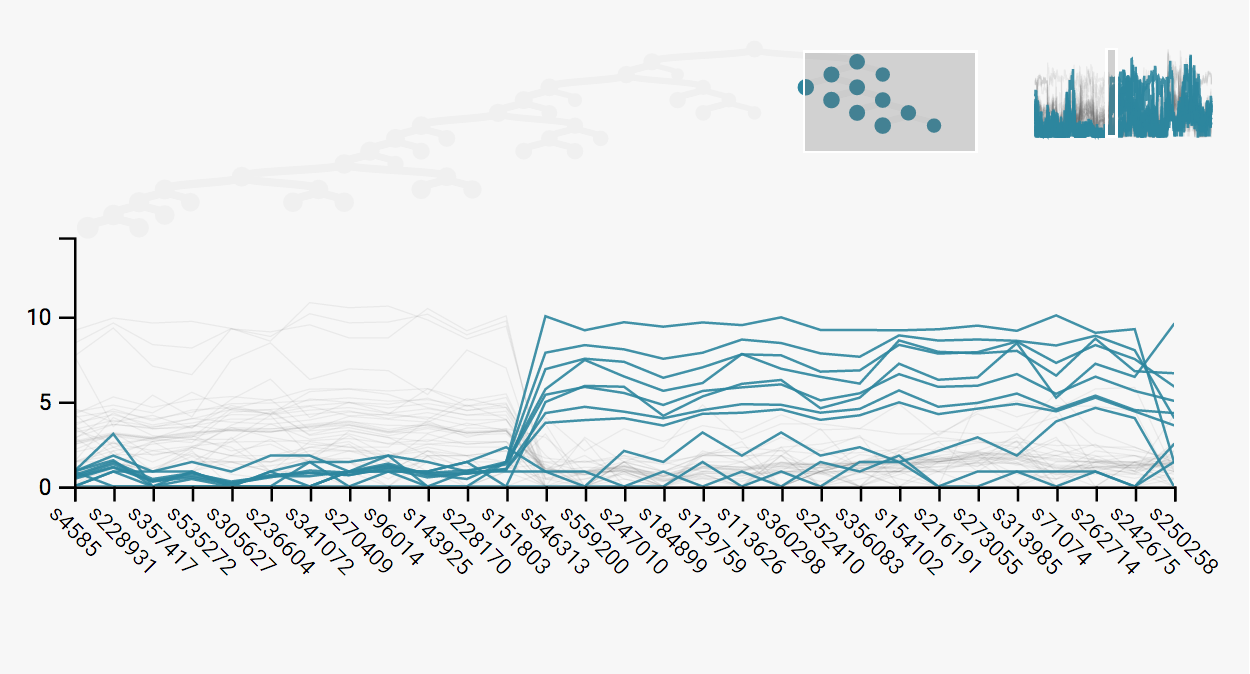
\includegraphics[width=225px]{figure/gp_cluster1}
    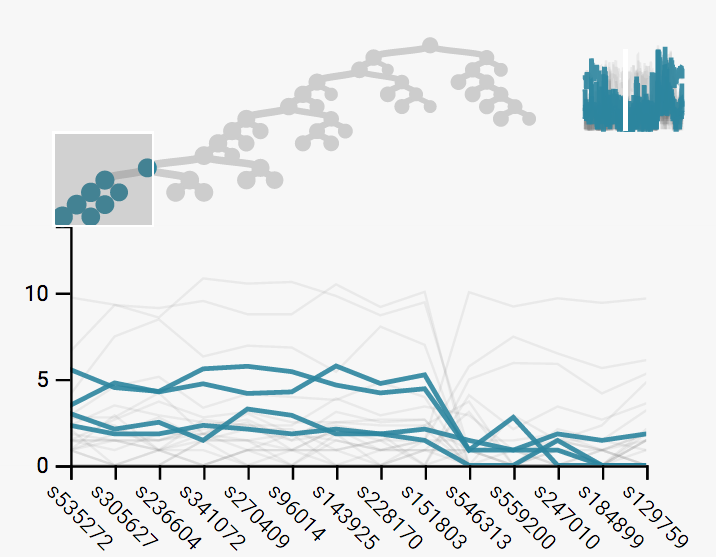
\includegraphics[width=225px]{figure/gp_cluster2}
}

\caption{An application to the Global Patterns demonstrates how linking in treelapse can be applied to combine hierarchical clustering and parallel coordinates views.}\label{fig:gptimebox}
\end{figure}

In Figure \ref{fig:gptimebox}, we compare two subclusters from the
hierarchical clustering tree, after zooming to a few of the bacteria
that distinguish between the clusters. Upon revisiting the original
data, it becomes clear that the samples highlighted on the left come
from freshwater samples, while those on the right come from soil and
skin, and looking up taxonomic groups associated with the distinguishing
bacteria confirms this. For example, many of the species with high
abundances in the left figure come from order Oceanospirillales.

\subsubsection*{Inspecting Confirmatory Analysis}\label{structssi}

In addition to facilitating exploratory study, treelapse has potential
value as a device for inspecting confirmatory analysis. We provide an
illustration extending an example from \citep{callahan2016bioconductor}, which
formally tested bacterial species for association with age in a sample of mice.
The testing approach advocated there is particularly well-suited to
visualization with treelapse, since it sought to detect associations at multiple
levels of phylogenetic resolution, using statistical tools developed in
\citep{yekutieli2008hierarchical, sankaran2014structssi}.

The data of interest in \citep{callahan2016bioconductor} are bacterial counts
collected across old and young mice. After variance-stabilizing these counts
using DESeq2 \citep{love2014moderated}, a $t$-test was
applied to each node in a phylogenetic tree, comparing abundances
between old and young mice. To account for multiple testing, we employ
the structSSI algorithm \citep{yekutieli2008hierarchical, sankaran2014structssi}
along with methods available in the \texttt{multtest} package
\citep{pollard2005multiple}.

To interpret the results, we apply timebox trees. Our goals are to (1)
identify subtrees with consistently elevated differential abundance
across age groups and (2) compare alternative multiple testing
adjustment procedures. Our approach is to display the negative-log raw
and adjusted $p$-values for each node, with alternative methods
compared via parallel coordinates. One view of the resulting display is
captured in Figure \ref{fig:structssi}. First, we see that significant
nodes tend to be significant across all methods -- the ordering between
different series appears stable. Interestingly, the Sidak one-step and
structSSI procedures seem to have lower power than the others, including
conservative FWER-controlling methods, like the Bonferroni procedure.
Further, in this application, FDR-controlling techniques do not seem to
offer notably different adjusted $p$-values, relative to those
controlling FWER. This suggests that, for this problem, bacteria are
either strongly associated with age, or not associated at all, so that
there is little gain from using more sensitive procedures.

\begin{figure}

{\centering 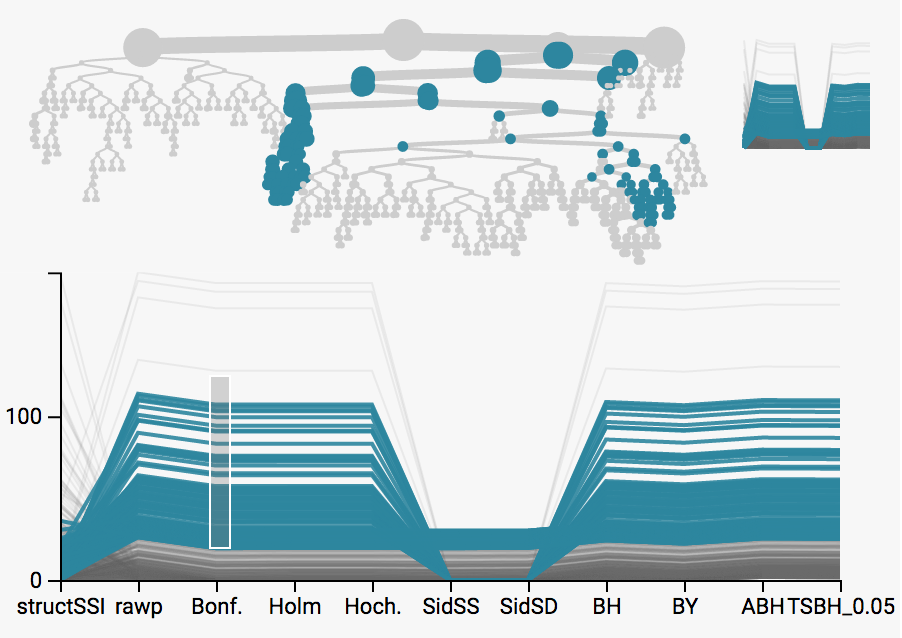
\includegraphics[width=250px]{figure/structssi}

}

\caption{Viewing a tree of $p$-values across different methods highlights two subtrees with strong associations with mouse age, across several testing procedures.}\label{fig:structssi}
\end{figure}

Further, selecting series with strong association between abundance and
age, two major subtrees are brought to the forefront. Separately
querying the the taxonomic identities of these bacteria reveals that they are
two subgroups of Clostridia, which is consistent with the analysis of
\citep{callahan2016bioconductor}. More than this specific analysis outcome, this
view demonstrates that interactive visual inspection of results from
confirmatory analysis provides deeper insight than the standard practice of
printing tables of (adjusted or unadjusted) $p$-values: the relationship between
significant nodes is only clear upon visualization on the tree.

\subsection*{Conclusion and Future Work}\label{conclusion}

Here, we have reviewed some fundamental principles of data visualization
and described their implementation in a new treelapse package. Further,
we have provided examples of the practical usefulness of these
principles in real-world data analysis situations.

This package has only developed basic ideas, and there are a number of
potentially useful extensions worth exploring. For example, we have not
considered the principle of arrangement in our visualizations
\citep{buja1996interactive},
though many of our conclusions were based on comparing alternative
selections of the same display. We could imagine faceting our displays
across groups to make these types of comparisons more accessible.
Further, we have only worked with the DOI distribution described in
\citep{heer2004doitrees}. It would be interesting to define a more statistical
notion of interest along nodes, based on cognostics, for example
\citep{hafen2013trelliscope, friedman2002john}. A simple extension could be to
allow graph layouts instead of trees in time and
treebox displays, for data that cannot be coerced into a hierarchical
structure. Finally, if these ideas turn out to be useful in practice, it
would be valuable to modularize the basic visualization layouts and
relationships into a library, allowing the wider community to construct
novel linked, interactive graphics with minimal effort.

In summary, we have built an easily accessible R package for
visualization techniques in a very specific methodology problem --
analysis of differential abundance and dynamics in hierarchically
structured data -- that appears in a variety of application domains. We
have leveraged a link between R and D3
\citep{vaidyanathan2014htmlwidgets} to create
visualizations during the exploratory phase of data analysis; in this
way our work is a departure from the culture of polished, journalistic
visualizations prioritized by the D3 community. Finally, we have given a
series of examples to demonstrate how the general visualization
techniques of focus-plus-context and linked brushing can be practically
incorporated into a range of practical analysis workflows, from studying
the impact of bacteria on human health to better allocating units in
commuter bikesharing systems.

\bibliographystyle{plainnat}
\bibliography{bibliography}

\end{document}
